\documentclass[10pt]{article} 
\usepackage{graphicx}
\usepackage[T1]{fontenc}
\usepackage{longtable}
\usepackage{mathtools}
\usepackage{fixltx2e}
\begin{document}
\title{Initial report on analysis of the Anganwadi 2010 dataset} 
\author{Avishek Sen Gupta\\ThoughtWorks}
\maketitle
\newpage
\tableofcontents
\listoffigures
\newpage

\section{Abstract}
This report summarises the results of exploration of the Anganwadi dataset provided by the Akshara Foundation. The analysis aims to characterise the structure of the data, and reveal trends (which would otherwise be obscured by the format of the source data) which may inform strategy through subsequent prediction and/or classification procedures.

\newpage
\section{Methodology}
\subsection{CRISP-DM}
\textbf{CRISP-DM} is a process model distilled from the most common approaches used in data mining procedures. It stands for Cross Industry Standard Process for Data Mining. Not so much a prescription as a collection of 'good practices' followed by data mining professionals, \textbf{CRISP-DM} has the following characteristics.

\begin{itemize}
\item Domain-neutral
\item Tool-neutral
\item Provides a structural approach to the data mining process
\end{itemize}

\textbf{CRISP-DM} segregates data mining endeavours into the following phases.

\begin{itemize}
\item Business Understanding
\item Data Understanding
\item Data Preparation
\item Modeling
\item Evaluation
\item Deployment
\end{itemize}

\subsection{Relevance of CRISP-DM to this report}
As far as this report is concerned, the relevant or most significant phases we focus on are:
\begin{itemize}
\item Data Understanding
\item Data Preparation
\item Modeling
\end{itemize}

Work on the Evaluation step is still preliminary, and will probably be the subject of another report. In a full-fledged project, the rest of the activities upstream and downstream to the above list will assume more importance, and require corresponding investment.

\newpage
\section{Data Preparation}
\subsection{Nature of the source data}
The dataset comes from the education domain. The source data is a file, with each line corresponding to a single student evaluation record. Roughly, there are 29000 records, prior to any data sanitisation. Each line is pipe(|)-delimited into multiple fields. The fields salient to this analysis are listed below:

\begin{itemize}
\item Location of the student's school
\item Language of the student
\item Student's score before intervention
\item Student's score after intervention
\end{itemize}

The score is not a single number, it is a set of 56 responses marked as 0/1. Generally, a 1 may be treated as a favourable answer, therefore, adding them up to get a single aggregate score has natural ordering: a sense of who did better. We reproduce two such records below, with the original formatting.\\\\
{\footnotesize
30915|YALLAMMANADODDI|KANNADA|1231468|Girl||1NoSection|Aug 2010 Assessment
|1|1|1|1|1|1|1|1|1|1|1|1|1|1|1|1|1|1|1|1|1|1|1|1|1|1|1|1|1|1|1|1|1|1|1|1|1|1|1|1|1|1|1|1|1|1|1|1|1|1|1|1|1|1|1|1
|Anganwadi Post Test|1|1|1|1|1|1|1|1|1|1|1|1|1|1|1|1|1|1|1|1|1|1|1|1|1|1|1|1|1|1|1|1|1|1|1|1|1|1|1|1|1|1|1|1|1|1|1|1|1|1|1|1|1|1|1|1|}\\

{\footnotesize 29607|BADAMAKAAN I|KANNADA|1445172|Girl|URDU|1NoSection|Aug 2010 Assessment
|1|0|1|1|0|1|0|1|1|1|1|1|1|1|1|0|1|1|1|1|1|0|1|1|1|1|1|0|1|1|1|0|1|1|1|1|1|1|0|1|1|0|1|1|1|1|1|1|1|1|1|1|1|1|1|0
|Anganwadi Post Test|1|0|1|1|1|0|1|1|0|1|1|0|1|1|1|1|0|1|1|1|0|0|1|1|0|1|0|0|1|1|1|0|1|1|0|0|1|1|1|0|0|1|1|1|1|1|1|1|1|1|1|1|1|1|1|1|
...
}\\

Looking at the second row, we see that the location of the Anganwadi is BADAMAKAAN I, the student is female and speaks Urdu. The first contiguous set of 0s and 1s is the pre-intervention score, and the next set is the post-intervention one.

\newpage
\subsection{Data representation}
\subsubsection{Data store}
Before any sort of sanitisation or analysis may be performed, it is important to ensure that the source data is stored in a format/datastore which makes querying and modifying the data relatively painless. This decision is largely driven by technological considerations, like:

\begin{itemize}
\item Scale of data (centralised/distributed store?)
\item Sophistication of queries (OLAP/OLTP?)
\item Structure of data, or lack thereof (SQL/NoSQL?)
\end{itemize}

We were dealing with only about 29000 records, and most of the analysis would probably be performed outside the database. Thus, we opted to use MySQL as our datastore.

\subsubsection{Schema}
The decisions when creating the database schema affect the ease of querying for relevant information. Apart from the attributes of interest, we wanted to store the individual binary responses as well. One way is to create one column for each response, giving us a total of 112 columns for storing these responses (56 for pre-intervention, 56 for post-intervention). The other way, and that is the one that we chose was to store this information as a 64-bit integer (bigint for MySQL). When required, we could unpack the individual response bits from this number.\\
A {\tt desc responses;} command on the table reveals the schema we ended up with.

{\tt
\begin{verbatim}
+------------------+------------+------+-----+---------+----------------+
| Field            | Type       | Null | Key | Default | Extra          |
+------------------+------------+------+-----+---------+----------------+
| student_id       | int(11)    | YES  |     | NULL    |                |
| area             | char(50)   | YES  |     | NULL    |                |
| pre_performance  | bigint(20) | YES  |     | NULL    |                |
| post_performance | bigint(20) | YES  |     | NULL    |                |
| language         | char(50)   | YES  |     | NULL    |                |
| gender           | char(20)   | YES  |     | NULL    |                |
| pre_total        | int(11)    | YES  |     | NULL    |                |
| post_total       | int(11)    | YES  |     | NULL    |                |
| id               | int(11)    | NO   | PRI | NULL    | auto_increment |
| school_id        | int(11)    | YES  |     | NULL    |                |
| year             | int(11)    | YES  |     | NULL    |                |
+------------------+------------+------+-----+---------+----------------+
\end{verbatim}
}

The most important use of the reference data is to locate the schools geographically. Given that geocoding the school from its name, we used the cluster to locate schools in 2D space. We deal with geographical analysis in a later section. The schema of the master data mostly mirrors the CSV master data file format, with the addition of latitude and longitude, like so:

{\tt
\begin{verbatim}
+-------------+----------------+------+-----+---------+----------------+
| Field       | Type           | Null | Key | Default | Extra          |
+-------------+----------------+------+-----+---------+----------------+
| district    | char(50)       | YES  |     | NULL    |                |
| block       | char(50)       | YES  |     | NULL    |                |
| cluster     | char(50)       | YES  |     | NULL    |                |
| school_id   | int(11)        | YES  |     | NULL    |                |
| school_code | char(20)       | YES  |     | NULL    |                |
| school_name | char(50)       | YES  |     | NULL    |                |
| id          | int(11)        | NO   | PRI | NULL    | auto_increment |
| latitude    | decimal(20,10) | YES  |     | NULL    |                |
| longitude   | decimal(20,10) | YES  |     | NULL    |                |
+-------------+----------------+------+-----+---------+----------------+
\end{verbatim}
}

To identify latitude and longitude, we used Google's Map API to geocode the cluster information. It is to be noted that there may be some clusters which weren't located by the Map API, and some more work is needed to cross-validate the coordinate information taken from the Map API.

\subsection{Data migration: Identifying invalid data}
It is natural to expect missing or corrupted data. The most crucial attribute are the score data, as any misinterpretation of that data may adversely bias the quality of our analysis. Thus, specific checks were put in place to ensure that none of the binary responses was null or some string other than 0 or 1.\\\\
Using this check, we found 1067 responses which violated it. All of them had either empty pre- or post-intervention scores. We did not migrate these response records, though it may be possible to do Monte Carlo simulations to predict the missing data.\\
As a result, out of a total of 28535 records in the original source, 27468 were migrated to the database.\\
We also found a large fraction of records which did not have a LANGUAGE attribute, i.e., that field was empty. Nevertheless, they were included in the migration.

\newpage
\section{Bias}
Analysis is most suscpetible to bias in the data collection stage. Sampling is one such activity. If, for a statistical study, participating individuals are not equally likely to have been selected, it may be difficult to distinguish between the actual phenomenon and this biased sampling.
This sort of bias is called sampling bias.

\newpage
\subsection{Sampling bias}
To find evidence for bias, we looked at a few parameters.
Here is the breakdown of the population by language, with the biggest language bucket highlighted.\\\\
Unspecified=869\\
URDU=3564\\
\textbf{KANNADA=18685}\\
TELUGU=1688\\
TAMIL=2051\\
MARATHI=91\\
OTHER=239\\
HINDI=243\\
KONKANI=18\\
GUJARATHI=12\\
NOT KNOWN=3\\
ORIYA=2\\
MULTI LNG=1\\
BENGALI=1\\
NEPALI=1\\
\\
There is an overwhelming proportion of students who speak Kannada as their mother tongue (leading by an order of magnitude), a fact that is very likely to bias any sort of analysis where language is involved. We must remain cognizant of such biases, and interpret the results accordingly.\\\\
Here is the breakdown of the population by gender.\\\\
\textbf{Girl=14822}\\
Boy=12646\\\\
There is not a huge disparity between the two sexes, which indicates that any analysis/prediction based on gender may be less biased.

\newpage
\section{Shape of the Data}
Before embarking on any deep analysis of data, it behooves us to look at the shape of the raw data. There are a few reasons why we want to do this.\\
\begin{itemize}
\item \textbf{Evident trends/outliers}: Visualisation of the raw data set is always a quick way to spot trends without doing too much analysis. Of course, visualisation is best suited for 1,2 and 3-dimensional data: data of higher dimensionality must usually be either sliced prior to visualisation, or have its dimensionality reduced, before projecting it onto the 2D plane.\\
Having said that, there are other ways of visualising the data without sacrificing any dimensions at all, such as Parallel Coordinates, though it is more suited to data exploration.
\item \textbf{Evidence of conformance to well-known distributions}: There exist many probability distributions, some of whose properties are well-studied and well-known, like the Normal distribution. If the data approximates one of these distributions, there are several mature statistical methods which may be applied to test different hypotheses and properties of the data.\\
Indeed, many of the classical statistical analyses make the assumption that the underlying data is (approximately) normally distributed.
\end{itemize}

In the following sections, we shall explore the shape of the Anganwadi 2010 dataset, and record our observations on it.

\subsection{Univariate distributions}
Figure~\ref{ShapeOfData} shows 3 distributions: the pre-intervention scores, the post-intervention scores, and the improvements.\\
\begin{figure}
\caption{Probability distributions of pre-, post-intervention, and improvement}
\label{ShapeOfData}
\begin{center}
	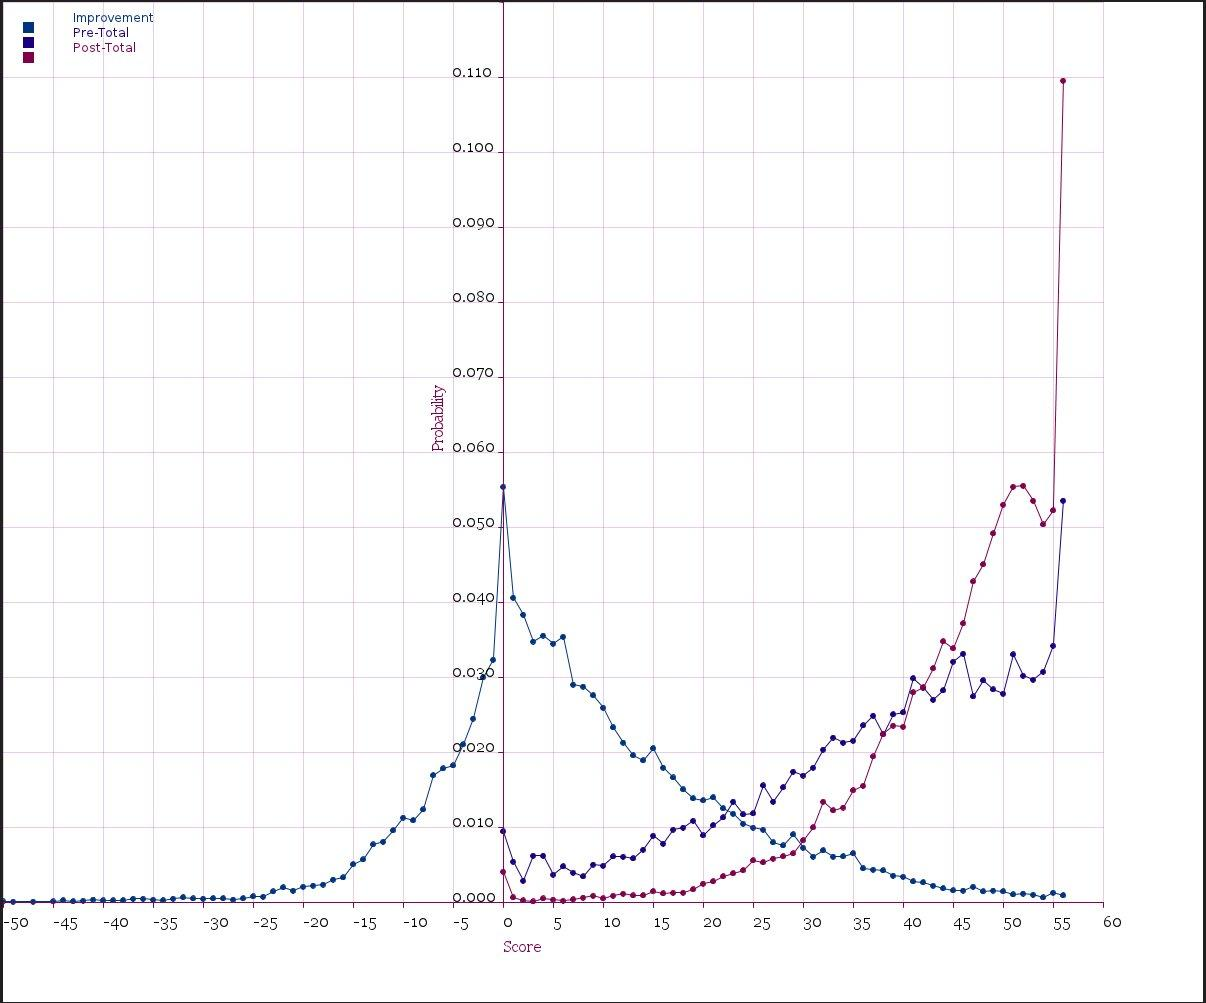
\includegraphics[width=160mm]{ReportMedia/ShapeOfData.jpg}
\end{center}
\end{figure}
\subsubsection{Observations/Notes}
\begin{itemize}
\item The pre-intervention score with the highest number of students is 56, which is the highest score possible. This implies that, even prior to intervention, a sizeable fraction of the students have scored very high on the test.
\item The post-intervention score also follows the same trend, albeit with a steeper curve, which implies that many students have scored better in the post-test than in the pre-test.
\item The improvement distribution is peaked, the peak being near zero. This makes sense, because if a large fraction of students answered all 56 questions as 1 in the pre-intervention score, there really is no way for them to improve. This is assuming that their performance did not worsen in the post-test. In fact, the calculated mean is around 7.
\item There is a significant fraction of students whose performance has worsened in the post-test. This number is 7081. Out of those, we noticed that the worsening was dramatic for a small set. We have listed down the records which had a regression of 40 or more, below.

{\tt
\begin{verbatim}
+------------+-----------------------+-----------+------------+----------+
| student_id | area                  | pre_total | post_total | language |
+------------+-----------------------+-----------+------------+----------+
|    1506619 | VABASANDRA            |        52 |          0 | KANNADA  |
|    1444355 | KITTAGANA COLONY      |        56 |          0 | KANNADA  |
|    1426910 | PRIYA DARSHINI        |        53 |          0 | KANNADA  |
|    1445387 | KYALASANAHALLI        |        51 |          1 | TELUGU   |
|    1445382 | KOTHANUR              |        44 |          0 | TAMIL    |
|    1445383 | KOTHANUR              |        41 |          0 | KANNADA  |
|    1442911 | BETTANA PALYA         |        55 |         12 | KANNADA  |
|    1445160 | KODIGEHALLI           |        52 |          0 | KANNADA  |
|    1457095 | KAVERI NAGARA         |        41 |          0 | KANNADA  |
|    1457090 | KAVERI NAGARA         |        44 |          0 | TELUGU   |
|    1457092 | KAVERI NAGARA         |        41 |          0 | TELUGU   |
|    1507686 | REHMATH NAGAR         |        44 |          0 | URDU     |
|    1448385 | MALSANDRA             |        50 |          0 | KANNADA  |
|    1455798 | KANTEERAVA COLONY     |        55 |         15 | KANNADA  |
|    1444466 | PRIYA DARSHINI        |        52 |          0 | KANNADA  |
|    1444467 | PRIYA DARSHINI        |        44 |          0 | KANNADA  |
|    1445337 | RACHENAHALLI          |        52 |          0 | KANNADA  |
|    1425269 | VINYAKNAGAR           |        41 |          0 | KANNADA  |
|     552534 | KYALASANAHALLI        |        52 |          1 | TELUGU   |
|    1448976 | KRISHNA SAGARA COLONY |        54 |         14 | KANNADA  |
|    1507157 | BELTHURU              |        52 |          7 | KANNADA  |
|    1444897 | MUNESHWARA NAGAR      |        45 |          0 | TAMIL    |
|    1444890 | MUNESHWARA NAGAR      |        40 |          0 | KANNADA  |
|    1542861 | VERABADRA NAGAR 1     |        56 |          1 | KANNADA  |
|    1358415 | KOTHANUR              |        48 |          8 |          |
|    1445437 | THRIVENINAGARA        |        40 |          0 | TELUGU   |
|    1442907 | BETTANA PALYA         |        55 |          8 | KANNADA  |
|    1457106 | KAVERI NAGARA         |        40 |          0 | TELUGU   |
|    1445444 | THRIVENINAGARA        |        41 |          0 | TELUGU   |
|    1444474 | PRIYA DARSHINI        |        54 |          0 | KANNADA  |
|    1445159 | KODIGEHALLI           |        41 |          0 | KANNADA  |
|     511998 | KODIGEHALLI           |        55 |          0 | KANNADA  |
|    1356274 | KAVERI NAGARA         |        56 |          0 |          |
|    1358429 | KOTHANUR              |        42 |          0 |          |
|    1497510 | JALAHALLI 1           |        42 |          0 | KANNADA  |
|    1443914 | BIDARAHALLI           |        56 |         12 | KANNADA  |
|    1366955 | PRIYA DARSHINI        |        53 |          0 | KANNADA  |
|    1366956 | PRIYA DARSHINI        |        53 |          0 | KANNADA  |
|    1447019 | MADAPPANA HALLI       |        42 |          0 | TELUGU   |
|    1355112 | BYRATHI BANDE         |        55 |         14 |          |
|    1504259 | MAYASANDRA  A         |        56 |          0 | KANNADA  |
|    1457120 | KAVERI NAGARA         |        43 |          0 | TAMIL    |
|    1457089 | KAVERI NAGARA         |        43 |          0 | TAMIL    |
|    1445171 | KODIGEHALLI           |        44 |          0 | KANNADA  |
|    1457203 | SARAIPALYA            |        51 |          0 | URDU     |
|    1457179 | BYRATHI BANDE         |        55 |         14 | KANNADA  |
|    1504538 | KEMPEGOWDA NAGAR      |        51 |          7 | KANNADA  |
|    1444486 | PRIYA DARSHINI        |        49 |          0 | KANNADA  |
|    1444488 | PRIYA DARSHINI        |        42 |          0 | KANNADA  |
|    1451831 | AMBED NAGAR           |        50 |          9 | TAMIL    |
+------------+-----------------------+-----------+------------+----------+
\end{verbatim}
}
\item The post-intervention score distribution seems to follow a power law. We shall consider modeling this attribute further on.
\end{itemize}
\subsection{Outlier analysis}

\subsection{Bivariate distribution}
So far, we've been looking at single variables in isolation. Figure~\ref{BivariatePrePost} shows a bivariate histogram of pre- vs. post-intervention scores. The lighter a cell, the more the number of records in that 'bucket'.\\\\
\begin{figure}
\caption{Bivariate probability distribution of pre- vs. post-intervention scores, with linear regression line $y = 0.224.x + 37.134$}
\label{BivariatePrePost}
\begin{center}
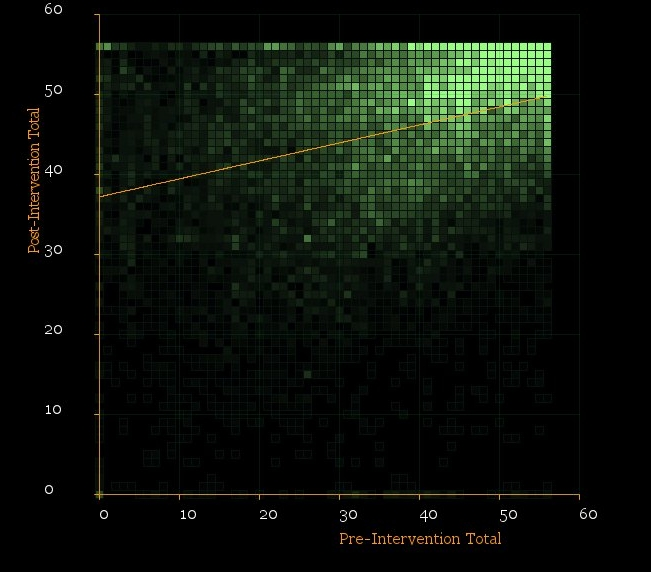
\includegraphics[width=160mm]{ReportMedia/BivariatePrePost.jpg}
\end{center}
\end{figure}
\subsubsection{Observations/Notes}
\begin{itemize}
\item Many of the scores seem to be clustered near the top right. To further highlight this, we have draw a linear regression line as a rough indicator of a trend (To model the trend in more detail, we could use LOESS). What is somewhat puzzling is that there are not a few students whose performance has dropped after the intervention. This is evident even without doing a linear regression.
\item The immediate outliers which are visible are the ones on the extreme left (pre~0, post~56) and at the origin (pre=0, post=0). The latter outlier(s) may be an artifact of corrupted data collection; we cannot say.
\end{itemize}

\subsection{Summary plots}
Summary plots are so called for their ability to summarise up a data set as a set of numbers, which can be easily interpreted. We used Box Plots to summarise the data, broken down by language. Figure~\ref{BoxPlotPrePost} shows that breakdown. The top row represents the box plots for the pre-intervention assessment, the bottom one for the post-intervention assessment.\\\\
\begin{figure}
\caption{Box plots of pre- and post-intervention scores, broken down by language}
\label{BoxPlotPrePost}
\begin{center}
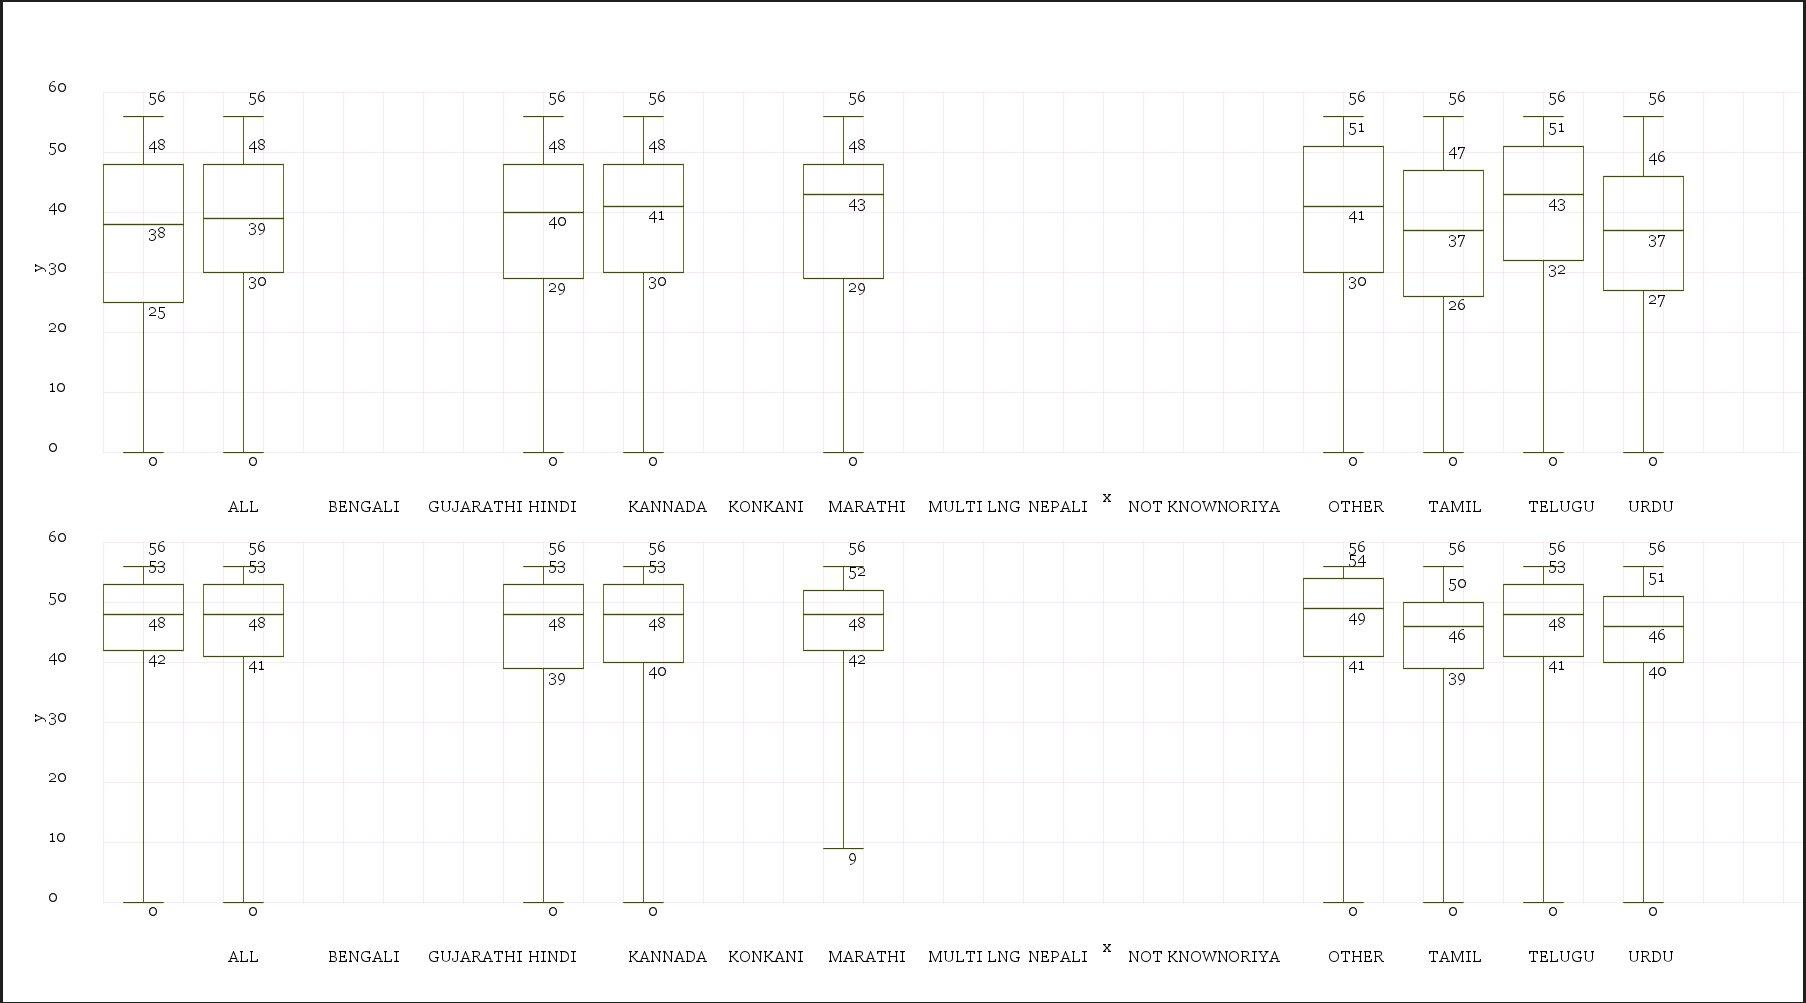
\includegraphics[width=160mm]{ReportMedia/BoxPlotPrePost.jpg}
\end{center}
\end{figure}
\subsubsection{Observations/Notes}
\begin{itemize}
\item Out of all the languages, we were not able to create box plots because the corresponding samples were too few in number to differentiate between the different quartiles. These languages are Bengali, MultiLng, Not Known and Oriya.
\item There are no dramatic differences between the plots in each set. The medians, 1st and the 2nd quartiles are rather close to each other.
\end{itemize}

\subsection{Rank Order Charts: Geoclusters}
One of the types of data that is pretty common is categorical nominal data. Categorical data is that which is non-numeric. Nominal data is that which does not lend itself to any intrinsic ordering. Names of places (if we ignore their coordinate system representation) are categorical data that is nominal.\\\\
The best way to summarise categorical data, especially if it is the Independent Variable, is to order records based on an ordinal Dependent Variable. This sort of a representation is called a Rank Order chart.
We have rank ordered the geographical clusters based on the student population in each cluster.
\newcounter{rownum}
\setcounter{rownum}{0}
\begin{longtable}{|c|c|c|c|}
	\hline
Index & Cluster &  Probability    &   Cumulative Distribution  \\
	\hline
\addtocounter{rownum}{1}\arabic{rownum}. & Sir M Vishweshwariah 1st Circle & 0.030690257754477937 & 0.030690257754477937 \\
\addtocounter{rownum}{1}\arabic{rownum}. & Sultanpalya & 0.030289791757681667 & 0.0609800495121596 \\
\addtocounter{rownum}{1}\arabic{rownum}. & konnana kunte & 0.02668559778651522 & 0.08766564729867482 \\
\addtocounter{rownum}{1}\arabic{rownum}. & kadugodi & 0.02584825979321392 & 0.11351390709188874 \\
\addtocounter{rownum}{1}\arabic{rownum}. & Laggere 4th circle & 0.025156545798747633 & 0.13867045289063637 \\
\addtocounter{rownum}{1}\arabic{rownum}. & K.R.Puram & 0.024756079801951363 & 0.16342653269258772 \\
\addtocounter{rownum}{1}\arabic{rownum}. & Murphy Town & 0.024064365807485073 & 0.1874908985000728 \\
\addtocounter{rownum}{1}\arabic{rownum}. & Netaji 2nd Circle & 0.02340905781272754 & 0.21089995631280034 \\
\addtocounter{rownum}{1}\arabic{rownum}. & Abbigere & 0.02326343381389253 & 0.23416339012669288 \\
\addtocounter{rownum}{1}\arabic{rownum}. & Begure & 0.023190621814475027 & 0.2573540119411679 \\
\addtocounter{rownum}{1}\arabic{rownum}. & Thavare kere & 0.022462501820299987 & 0.2798165137614679 \\
\addtocounter{rownum}{1}\arabic{rownum}. & Kodihalli & 0.022244065822047472 & 0.30206057958351534 \\
\addtocounter{rownum}{1}\arabic{rownum}. & Dodda Banaswadi & 0.02202562982379496 & 0.3240862094073103 \\
\addtocounter{rownum}{1}\arabic{rownum}. & Jigani & 0.021952817824377458 & 0.3460390272316878 \\
\addtocounter{rownum}{1}\arabic{rownum}. & Koramangala & 0.021370321829037427 & 0.3674093490607252 \\
\addtocounter{rownum}{1}\arabic{rownum}. & Byrathi & 0.020387359836901122 & 0.3877967088976263 \\
\addtocounter{rownum}{1}\arabic{rownum}. & Rajanakunte & 0.020059705839522355 & 0.4078564147371487 \\
\addtocounter{rownum}{1}\arabic{rownum}. & Varthur & 0.01944080384447357 & 0.42729721858162223 \\
\addtocounter{rownum}{1}\arabic{rownum}. & Hebbagodi & 0.01907674384738605 & 0.4463739624290083 \\
\addtocounter{rownum}{1}\arabic{rownum}. & Hreohalli & 0.018639871850881024 & 0.4650138342798893 \\
\addtocounter{rownum}{1}\arabic{rownum}. & Yalahanka & 0.01802096985583224 & 0.48303480413572153 \\
\addtocounter{rownum}{1}\arabic{rownum}. & Banashankari & 0.017438473860492208 & 0.5004732779962138 \\
\addtocounter{rownum}{1}\arabic{rownum}. & K Gollahalli & 0.0172928498616572 & 0.517766127857871 \\
\addtocounter{rownum}{1}\arabic{rownum}. & Sarjapura & 0.017183631862530944 & 0.5349497597204019 \\
\addtocounter{rownum}{1}\arabic{rownum}. & Mallasandra & 0.01711081986311344 & 0.5520605795835154 \\
\addtocounter{rownum}{1}\arabic{rownum}. & Kodigenahalli & 0.01689238386486093 & 0.5689529634483763 \\
\addtocounter{rownum}{1}\arabic{rownum}. & kasaba & 0.01667394786660842 & 0.5856269113149848 \\
\addtocounter{rownum}{1}\arabic{rownum}. & Haragadde & 0.016564729867482163 & 0.6021916411824669 \\
\addtocounter{rownum}{1}\arabic{rownum}. & Makali & 0.016455511868355904 & 0.6186471530508229 \\
\addtocounter{rownum}{1}\arabic{rownum}. & Doddakannelli & 0.016419105868647154 & 0.63506625891947 \\
\addtocounter{rownum}{1}\arabic{rownum}. & Mahantalingapura & 0.016200669870394643 & 0.6512669287898646 \\
\addtocounter{rownum}{1}\arabic{rownum}. & Baglur & 0.015836609873307123 & 0.6671035386631717 \\
\addtocounter{rownum}{1}\arabic{rownum}. & chandapura & 0.015836609873307123 & 0.6829401485364789 \\
\addtocounter{rownum}{1}\arabic{rownum}. & Bettahalasuru & 0.015690985874472114 & 0.698631134410951 \\
\addtocounter{rownum}{1}\arabic{rownum}. & Hesaragatta & 0.015690985874472114 & 0.7143221202854232 \\
\addtocounter{rownum}{1}\arabic{rownum}. & Kaggalipura & 0.0154725498762196 & 0.7297946701616428 \\
\addtocounter{rownum}{1}\arabic{rownum}. & Sondekoppa & 0.015217707878258336 & 0.7450123780399012 \\
\addtocounter{rownum}{1}\arabic{rownum}. & Wilson Garden & 0.01510848987913208 & 0.7601208679190332 \\
\addtocounter{rownum}{1}\arabic{rownum}. & Dommasanddra & 0.01510848987913208 & 0.7752293577981653 \\
\addtocounter{rownum}{1}\arabic{rownum}. & Kithuru Rani Channamma 3rd Circle & 0.01474442988204456 & 0.7899737876802099 \\
\addtocounter{rownum}{1}\arabic{rownum}. & Triveni 5th Circle & 0.014489587884083296 & 0.8044633755642931 \\
\addtocounter{rownum}{1}\arabic{rownum}. & Palace Guttalli Circle & 0.014453181884374545 & 0.8189165574486676 \\
\addtocounter{rownum}{1}\arabic{rownum}. & Kengeri circle & 0.014343963885248289 & 0.8332605213339159 \\
\addtocounter{rownum}{1}\arabic{rownum}. & Yashwanthpura & 0.014052715887578273 & 0.8473132372214942 \\
\addtocounter{rownum}{1}\arabic{rownum}. & Kuvempunagar 4th Circle & 0.013543031891655745 & 0.8608562691131499 \\
\addtocounter{rownum}{1}\arabic{rownum}. & Chikkajala & 0.012960535896315713 & 0.8738168050094657 \\
\addtocounter{rownum}{1}\arabic{rownum}. & Kadugondanahalli & 0.012596475899228193 & 0.8864132809086939 \\
\addtocounter{rownum}{1}\arabic{rownum}. & Attibele & 0.012523663899810689 & 0.8989369448085045 \\
\addtocounter{rownum}{1}\arabic{rownum}. & Indlavadi & 0.012341633901266929 & 0.9112785787097715 \\
\addtocounter{rownum}{1}\arabic{rownum}. & Sonnenahali & 0.012305227901558177 & 0.9235838066113297 \\
\addtocounter{rownum}{1}\arabic{rownum}. & Uttrahalli & 0.012232415902140673 & 0.9358162225134703 \\
\addtocounter{rownum}{1}\arabic{rownum}. & Machohalli & 0.012159603902723169 & 0.9479758264161935 \\
\addtocounter{rownum}{1}\arabic{rownum}. & Gavipura Guttahalli & 0.009210717926314256 & 0.9571865443425077 \\
\addtocounter{rownum}{1}\arabic{rownum}. & Marasur & 0.009137905926896752 & 0.9663244502694045 \\
\addtocounter{rownum}{1}\arabic{rownum}. & Netravathi & 0.00906509392747925 & 0.9753895441968837 \\
\addtocounter{rownum}{1}\arabic{rownum}. & Gopalapura & 0.008955875928352992 & 0.9843454201252367 \\
\addtocounter{rownum}{1}\arabic{rownum}. & Hennagara & 0.00873743993010048 & 0.9930828600553372 \\
\addtocounter{rownum}{1}\arabic{rownum}. & PANTHARAPALYA & 0.002621231979030144 & 0.9957040920343674 \\
\addtocounter{rownum}{1}\arabic{rownum}. & YARUB NAGAR & 0.001783893985728848 & 0.9974879860200963 \\
\addtocounter{rownum}{1}\arabic{rownum}. & VERABADRA NAGAR & 0.001310615989515072 & 0.9987986020096113 \\
\addtocounter{rownum}{1}\arabic{rownum}. & Yalahanka upnagar & 0.00043687199650502403 & 0.9992354740061163 \\
\addtocounter{rownum}{1}\arabic{rownum}. & DODDA BANASAWADI & 0.000400465996796272 & 0.9996359400029126 \\
\addtocounter{rownum}{1}\arabic{rownum}. & ASHRAYA NAGAR & 0.00036405999708752004 & 1.0 \\
\hline
\end{longtable}
\subsubsection{Observations/Notes}
\begin{itemize}
\item Out of 63 clusters, the top 38 clusters account for 75\% of the population.
\end{itemize}

\newpage
\section{Data Analysis and Exploration}
There are multiple ways of exploring datasets when simple visual inspection is tedious and unintuitive. Many of them are standard, but some of them may reveal more about the nature of the data. Often, they are motivated by specific business drivers and questions, and some exploration may be custom to the dataset under analysis. Data exploration is also commonly done through queries to an OLAP database.
\subsection{Parallel Coordinates}
Parallel coordinates are an interesting way to explore high-dimensional data without discarding any detail. The only downside is that the elegance of presentation is somewhat sacrificed.\\
Essentially, instead of aligning axes in orthogonal directions (we can visualise only upto 3), the axes are stacked horizontally, giving the impression of n parallel lines. A single data point in this n-dimensional representation is a set of broken lines spanning the widths between the axes.\\\\
The way to explore this visualisation is to highlight the samples of interest, based on some criteria. The highlighted samples can then be inspected visually to discover trends, if any. Figure~\ref{ParallelCoordinates} shows an example of exploration using parallel coordinates on the Anganwadi data.
\begin{figure}
\caption{Parallel Coordinates showing language, gender, school, pre- and post-intervention scores}
\label{ParallelCoordinates}
\begin{center}
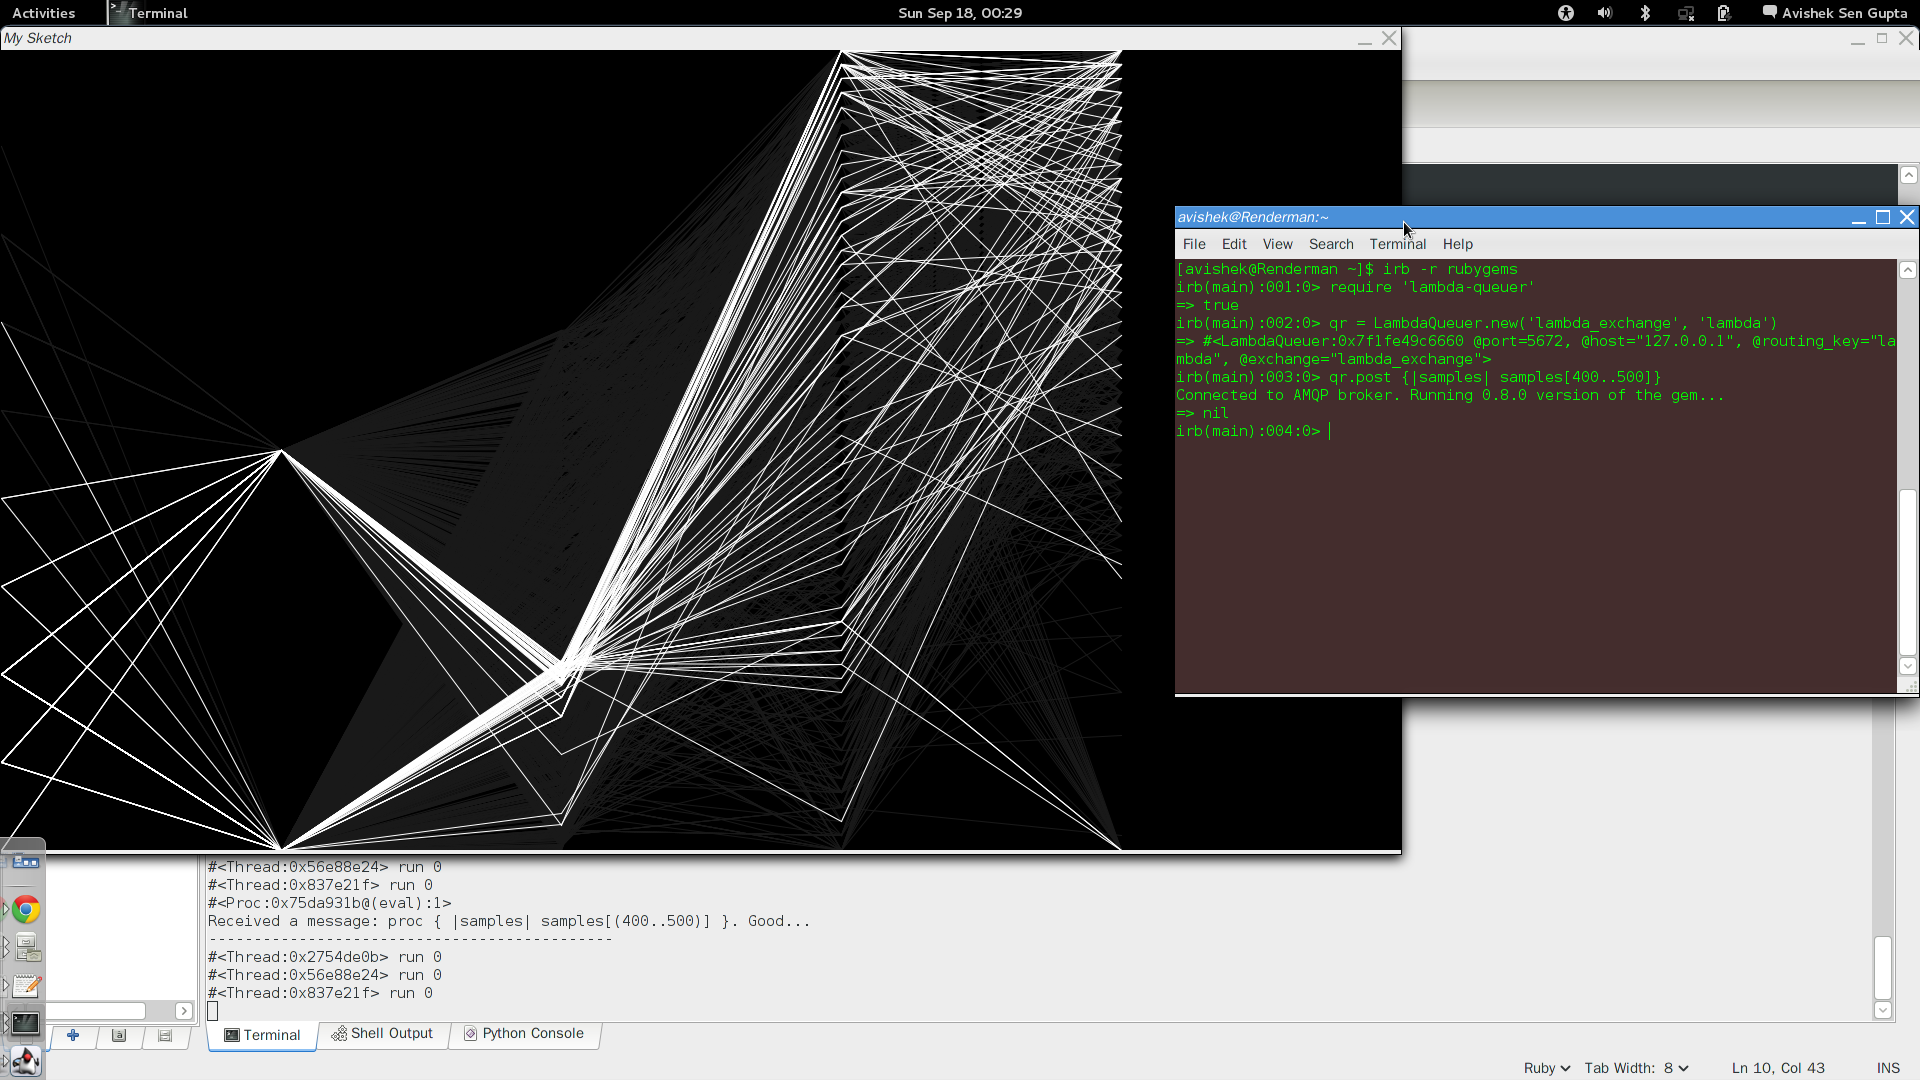
\includegraphics[width=150mm]{ReportMedia/ParallelCoordinates.jpg}\\
\end{center}
\end{figure}
\subsection{Covariance plot}
The covariance plot is a first step towards looking at the correlations between responses to individual questions. Basically, the kind of question such analysis can answer is, for example, how dependent is a response to question 40 on the response to question 3? Do they change together, i.e., is there a strong dependency between answer to question X and the answer to question Y?\\\\
Figure~\ref{CovariancePre} shows the covariance plot for the pre-intervention responses.\\
Figure~\ref{CovariancePost} shows the covariance plot for the post-intervention responses.\\
\begin{figure}
\caption{Covariance plot of pre-intervention responses}
\label{CovariancePre}
\begin{center}
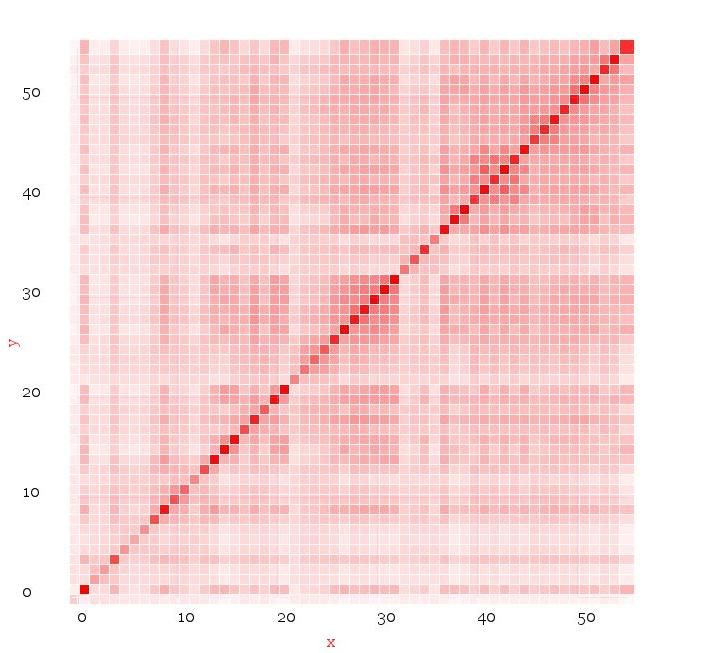
\includegraphics[width=120mm]{ReportMedia/CovariancePre.jpg}\\
\end{center}
\end{figure}

\begin{figure}
\caption{Covariance plot of post-intervention responses}
\label{CovariancePost}
\begin{center}
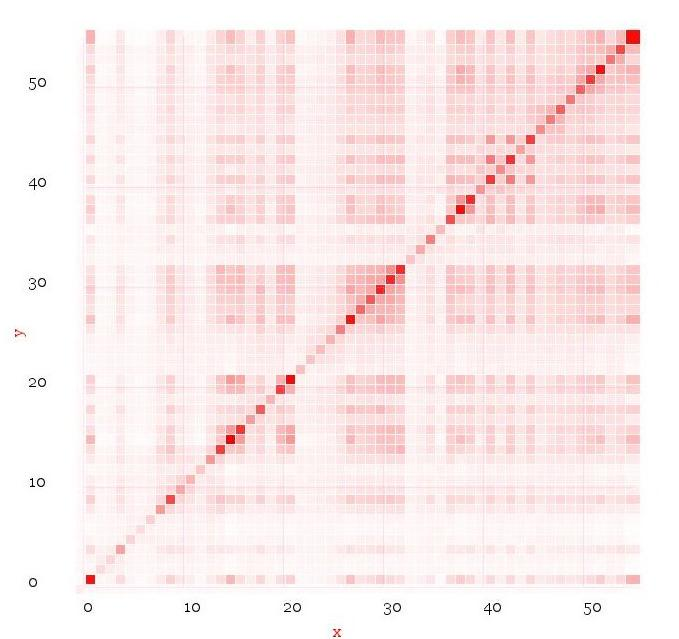
\includegraphics[width=120mm]{ReportMedia/CovariancePost.jpg}\\
\end{center}
\end{figure}
\subsubsection{Observations/Notes}
\begin{itemize}
\item The plots are color coded such that the darker the hue, higher the covariance. The plot is symmetric about the diagonal, and the diagonal is much darker because it is essentially the covariance of a single response with itself. The data has not been normalised yet, hence the diagonal hues vary.
\item The covariance between the responses appears weakened in the post-intervention scores, indicating that the degree of dependence between the responses has decreased.
\item There appear to be clusters of relatively high covariance, for example, between the questions in the range of (40-43), (26-31), etc. Further investigation may be needed to answer specific questions in this area.
\item Correlation does not imply causation. Inferred links between responses may be result of a deeper phenomenon; thus a high covariance doesn't necessarily imply a direct causative link between two responses.

\end{itemize}

\subsection{Geographical distribution}
\begin{figure}
\caption{Geocoded populations by cluster}
\label{GeographicalDistributionOfPopulation}
\begin{center}
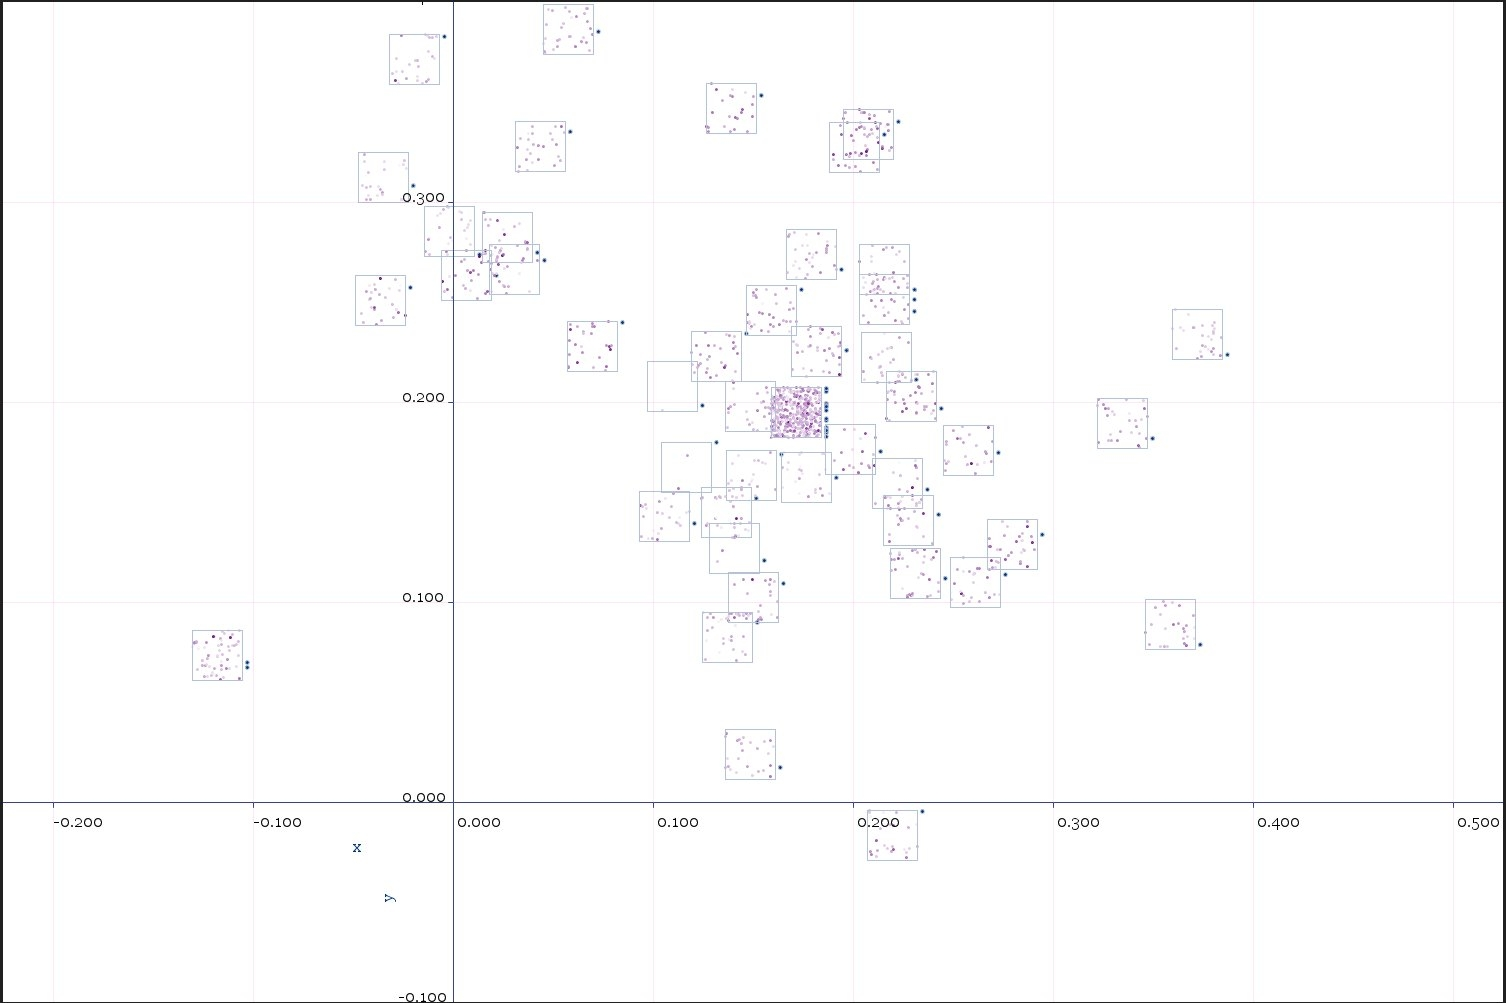
\includegraphics[width=170mm]{ReportMedia/GeographicalDistributionOfPopulation.jpg}\\
\end{center}
\end{figure}
\section{Models and Statistical Tests}
Models are simplified descriptions of the real-world phenomena, based on simplifying assumptions. Their primary use is to explain variations in observed data, and hopefully make useful predictions about data yet unseen.\\
Statistical tests, on the other hand, are designed to test certain hypotheses which might be inferred from the data set. These hypotheses may be proved or disproved by these tests, based on the notion of 'statistically significance'.\\ 
This section summarises the models and tests we've applied to the Anganwadi dataset.
\subsection{Tests for conformance to distributions}
Many of the tests in statistics work under the assumption that the underlying dataset (with or without transformation) is normally distributed, i.e., it follows a Gaussian probability distribution, namely:\\
\[f(x) = a e^ {\frac{(x-b)^2}{2c^2}}\]
This verification is important because it dictates, to a great extent, the validity of any tests we run. If the data turns out to be not normal, we will probably want to use nonparametric methods, which do not make assumptions about the shape of the distribution.
\subsubsection{Jarque-Bera test}
The Jarque-Bera test measures the conformance of a dataset to a Gaussian distribution using its skewness and kurtosis. For reference, the Jarque-Bera statistic is given by:\\

\[{JB}=\frac{n}{6} \left( S^2 + \frac14 (K-3)^2 \right)\]
where S (skew) and K (kurtosis) are defined as:

\[S = \frac{ \hat{\mu}_3 }{ \hat{\sigma}^3 } 
        = \frac{\frac1n \sum_{i=1}^n (x_i-\bar{x})^3} {\left(\frac1n \sum_{i=1}^n (x_i-\bar{x})^2 \right)^{3/2}}\]
\[
K = \frac{ \hat{\mu}_4 }{ \hat{\sigma}^4 }  
        = \frac{\frac1n \sum_{i=1}^n (x_i-\bar{x})^4} {\left(\frac1n \sum_{i=1}^n (x_i-\bar{x})^2 \right)^2}
\]
The null hypothesis that this statistic tests is that the skewness and excess kurtosis are both zero, which is the defining characteristic of a Gaussian distribution. The data below summarises the JB statistics for the pre-, post-intervention scores and the score improvements. Please note that the statistics from the data before the removal of the invalid data. This does not affect the results overmuch, however.\\\\
\textbf{Pre-intervention Score}\\
n = 28535
Skewness = -1.0001504234198\\
Kurtosis = -1.99959305171352\\
JB statistic = 34476.3843030411\\
\textbf{Conclusion : Pre-intervention scores are not normally distributed.}\\\\
\textbf{Post-intervention Score}\\
n = 28535\\
Skewness = -1.00010106352368\\
Kurtosis = -1.9997273050813\\
JB statistic = 34477.5108572449\\
\textbf{Conclusion : Post-intervention scores are not normally distributed.}\\\\
\textbf{Score Improvement}\\
n = 28535\\
Skewness = -4.24685767755943\\
Kurtosis = 37.1765663807246\\
JB statistic = 1474523.40413686\\
\textbf{Conclusion : Score improvements are not normally distributed.}\\\\
The initial probability distributions provided very clear evidence that the pre- and post-intervention scores were not normal: this is merely validation. However, the test also shows that the improvement is not normally distributed either.\\
If we notice the improvement distribution in Figure~\ref{ShapeOfData}, we notice a few things:
\begin{itemize}
\item Fat tails
\item Thin narrow peak (high kurtosis)
\item Fair amount of skew (Non-zero excess skew)
\end{itemize}

We did attempt to assess the visual fit of a Gaussian distribution, but this was not very successful. Figures \ref{ShapeOfImprovementWrtNormal} and \ref{ShapeOfTranslatedLogOffImprovementWrtCauchy} show some of our attempts at fitting different theoretical distributions. The Cauchy distribution was a closer fit after a translation and a transform, but there are still outliers.
\begin{figure}
\caption{Improvement data overlaid with theoretical Gaussian (${\sigma}^2$=245.47, $\bar{x}$= 7.22)}
\label{ShapeOfImprovementWrtNormal}
\begin{center}
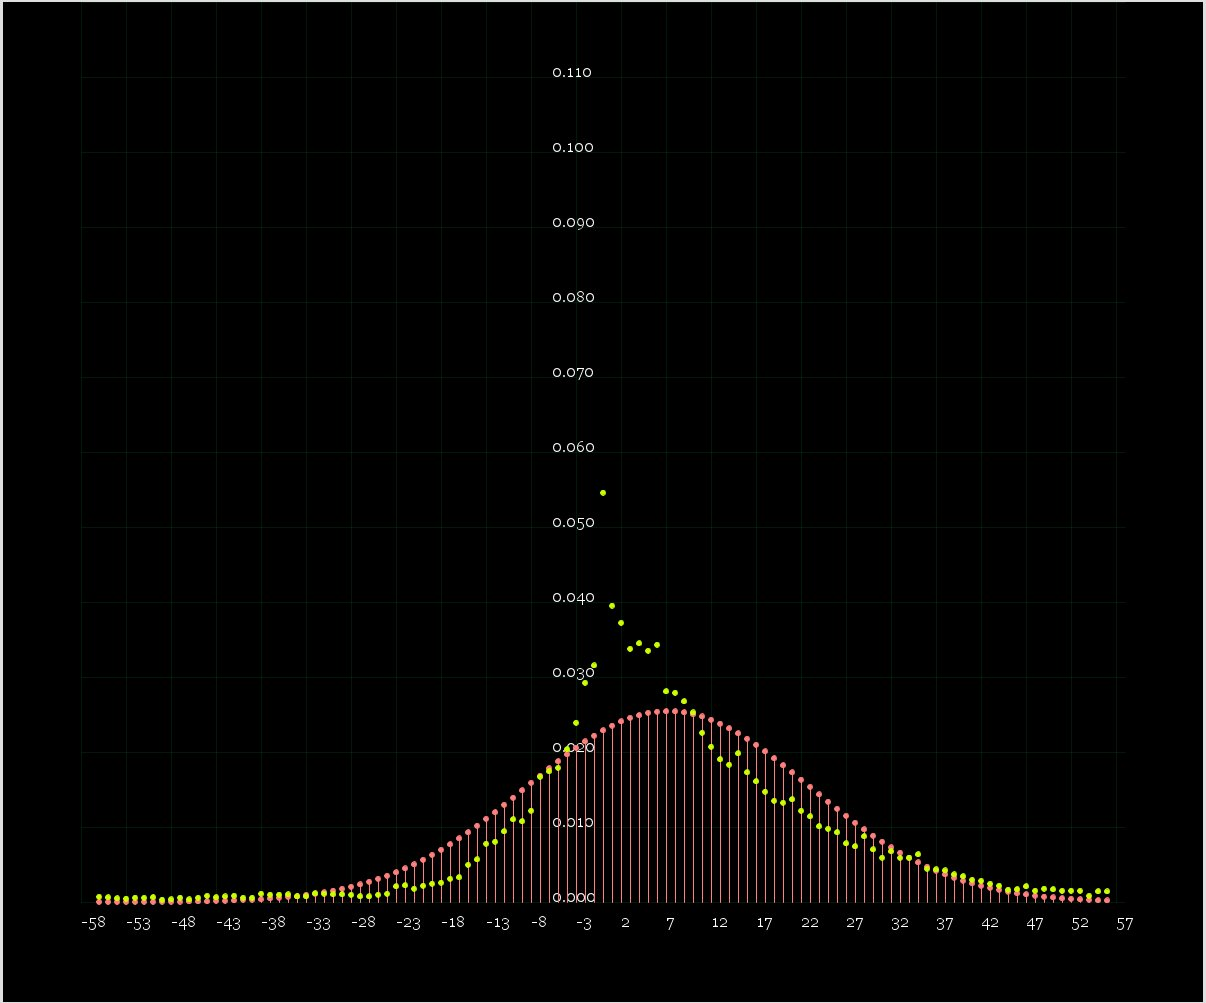
\includegraphics[width=120mm]{ReportMedia/ShapeOfImprovementWrtNormal.jpg}\\
\end{center}
\end{figure}

\begin{figure}
\caption{Translated log of data overlaid with theoretical Cauchy (scale=0.14, $\bar{x}$= 4.13)}
\label{ShapeOfTranslatedLogOffImprovementWrtCauchy}
\begin{center}
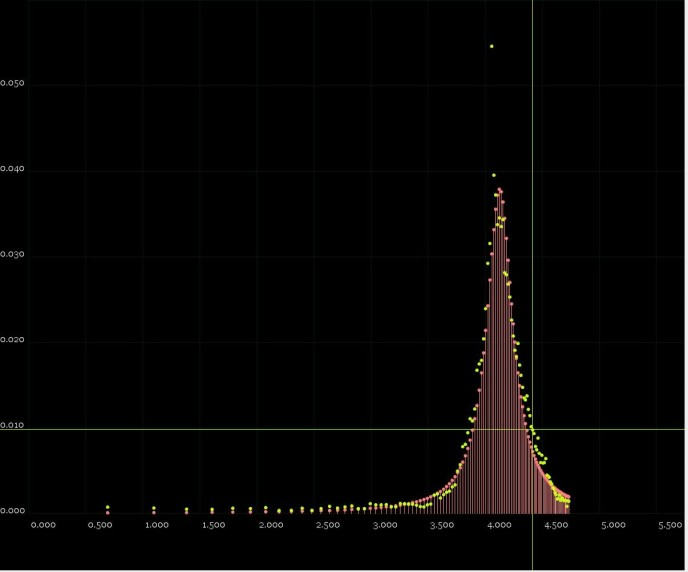
\includegraphics[width=120mm]{ReportMedia/ShapeOfTranslatedLogOffImprovementWrtCauchy.jpg}\\
\end{center}
\end{figure}
\subsubsection{Quantile-Quantile plots}
There is a visually more intuitive way of measuring the goodness of fit of a dataset to any theoretical probability distribution. That method is called a Quantile-Quantile plot. They are points marked off at regular intervals on the cumulative distribution function of a random variable. The Q-Q plot is so named for the two quantile plots that are reflected in a single plot: one for the theoretical distribution, and one for the dataset.\\
The theoretical distribution's quantile plot comes out as a straight line. If the dataset follows the distribution closely, it will also follow this line, more or less. Significant deviations indicate violation of fit. Figure~\ref{NormalProbabilityPlotImprovement} shows the Q-Q plot of score improvement and the Gaussian.
\begin{figure}
\caption{Quantile-Quantile plot of score improvement vs. theoretical Gaussian}
\label{NormalProbabilityPlotImprovement}
\begin{center}
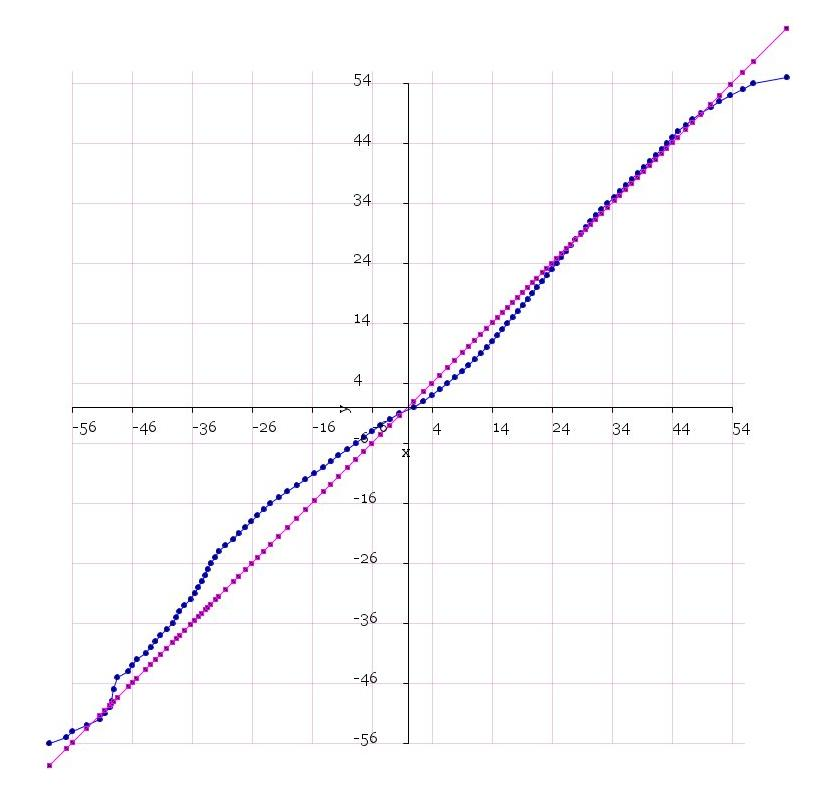
\includegraphics[width=120mm]{ReportMedia/NormalProbabilityPlotImprovement.jpg}\\
\end{center}
\end{figure}
\subsubsection{Observations/Notes}
\begin{itemize}
\item The dataset shows a systematic deviation from the Gaussian quantile.
\item Conformance to the theoretical distribution is never exactly possible, so the "fat pencil test" is used. Essentially, if the blunt end of a pencil covers both the theoretical and the actual dataset, we can say that the data approximates the model somewhat. In this case, the fat pencil test fails too.
\end{itemize}

We present another example of curve fitting to derive a probability distribution model, this time, with more success. We attempted to fit the exponential distribution to the post-intervention data. The exponential distribution is given as:
\[f(x,\lambda)=\left\{\begin{matrix}
 & {\lambda}e^{-{\lambda}x} &if x \geq 0\\ 
 & 0 &if x < 0\\
\end{matrix}\right.\]
Because improvement can be negative is well, we applied the following transform to the data:
\[I'(x)=I(x) + 57\]
As Figure~\ref{ExponentialProbabilityPost} shows, the distribution is a reasonable fit to the data.
\begin{figure}
\caption{Curve-fitted theoretical exponential for reflected post-intervention probability distribution}
\label{ExponentialProbabilityPost}
\begin{center}
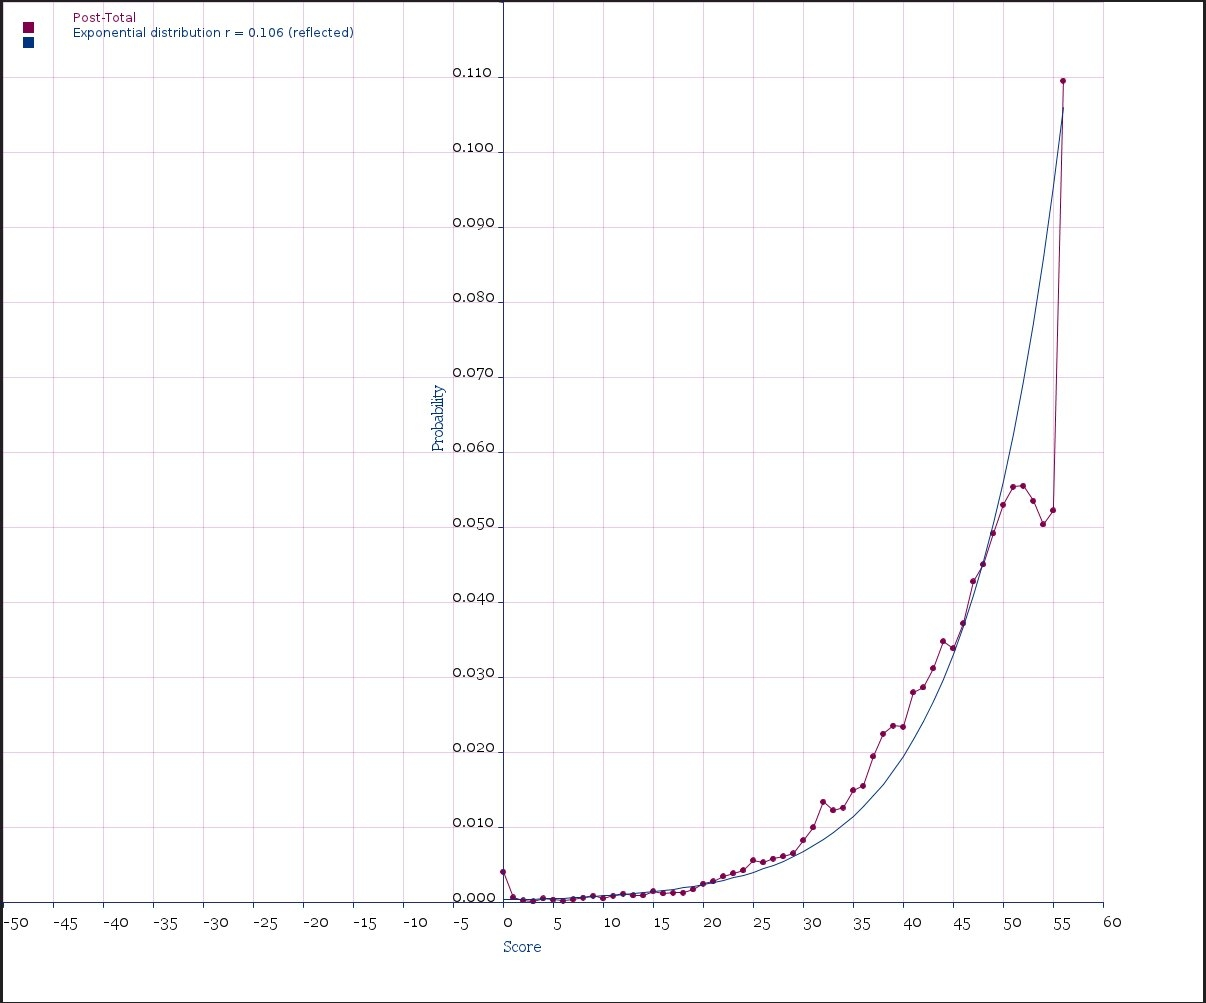
\includegraphics[width=160mm]{ReportMedia/ExponentialProbabilityPost.jpg}\\
\end{center}
\end{figure}
Further validation comes from the Q-Q plot of the dataset and the theoretical exponential in Figure~\ref{QQPlotPostVsExponential}. Note how closely the dataset tracks the theoretical quantile, except near the top right, which is where the 'kink' in the data set lies.
\begin{figure}
\caption{Quantile-Quantile plot of post-intervention score (reflected) vs. theoretical exponential}
\label{QQPlotPostVsExponential}
\begin{center}
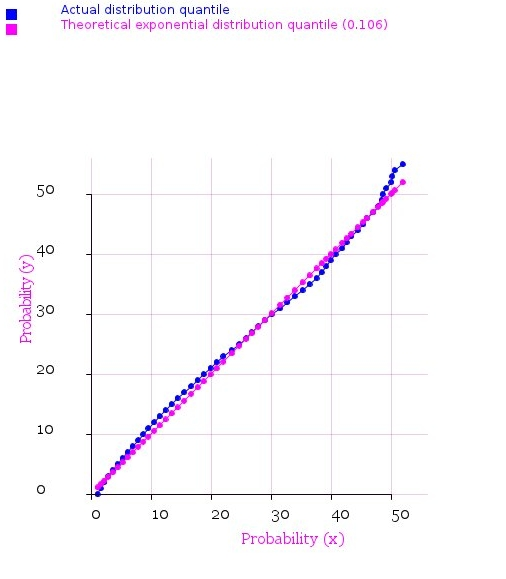
\includegraphics[width=120mm]{ReportMedia/QQPlotPostVsExponential.jpg}\\
\end{center}
\end{figure}

\subsection{The Central Limit Theorem}
Fortunately, we need not discard classical statistical techniques because the underlying distribution is not normally distributed. This is because even though the data itself is non-normal, its means are very probably normally distributed, regardless of the original distribution of the data.\\
This statement is known as the Central Limit Theorem, which states that:\\\\
\textbf{The distribution of the sum of a large number of independent, identically distributed variables will be approximately normal, regardless of the underlying distribution.}\\\\
To illustrate the point, we show the histograms of the means of the pre-intervention scores, post-intervention scores, and the improvements, in Figures \ref{CentralLimitTheoremPreTotal}, \ref{CentralLimitTheoremPostTotal}, and \ref{CentralLimitTheoremImprovement}, respectively.\\
The Jarque-Bera statistics for these three cases is well below the threshold. The shape validates that, too.
\begin{figure}
\caption{Central Limit Theorem illustration on the pre-intervention score}
\label{CentralLimitTheoremPreTotal}
\begin{center}
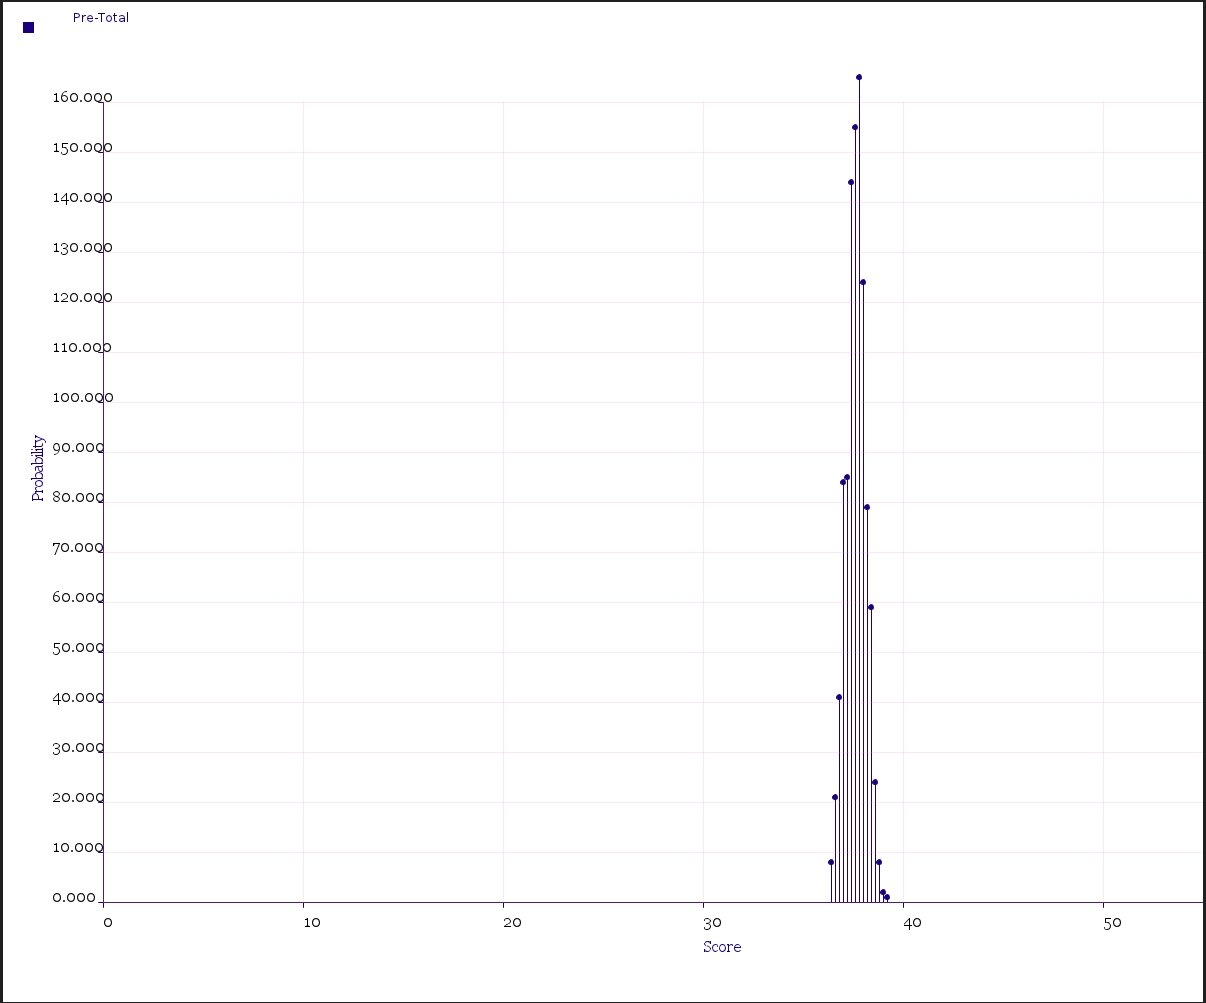
\includegraphics[width=90mm]{ReportMedia/CentralLimitTheoremPreTotal.jpg}\\
\end{center}
\end{figure}

\begin{figure}
\caption{Central Limit Theorem illustration on the post-intervention score}
\label{CentralLimitTheoremPostTotal}
\begin{center}
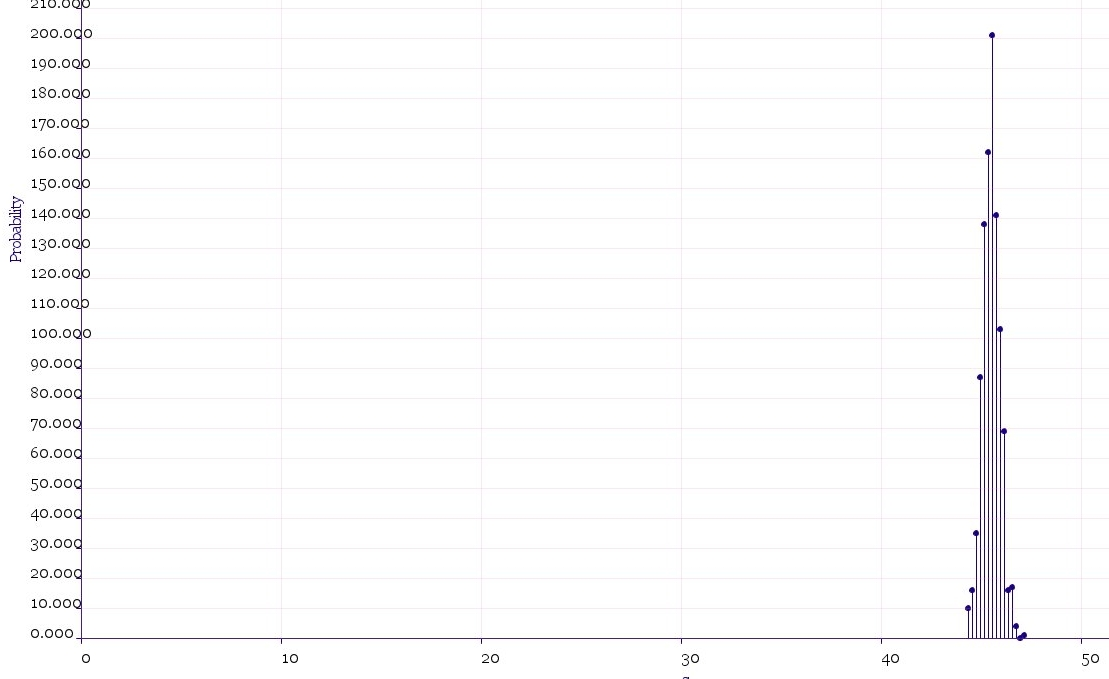
\includegraphics[width=90mm]{ReportMedia/CentralLimitTheoremPostTotal.jpg}\\
\end{center}
\end{figure}

\begin{figure}
\caption{Central Limit Theorem illustration on the improvement metric}
\label{CentralLimitTheoremImprovement}
\begin{center}
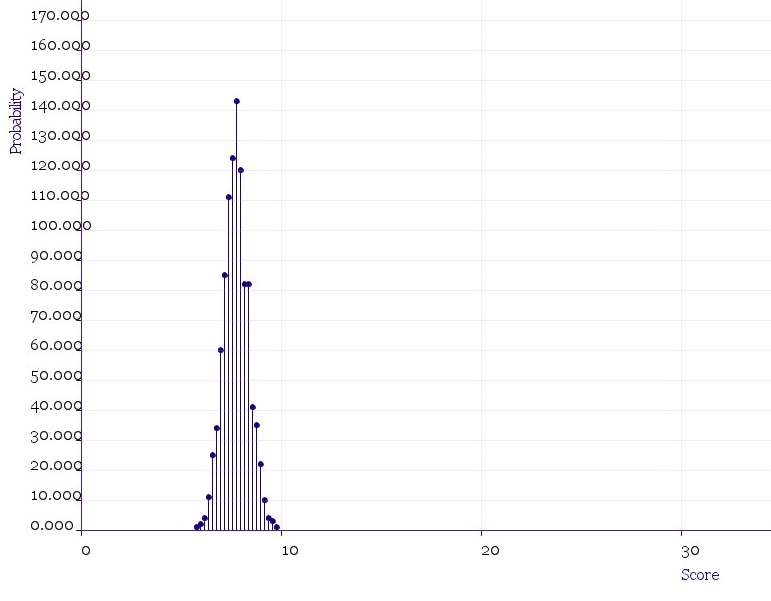
\includegraphics[width=90mm]{ReportMedia/CentralLimitTheoremImprovement.jpg}\\
\end{center}
\end{figure}
Why is the Central Limit Theorem important? It is because, even though statistical tests might not be appropriate for the raw, non-normal, data itself, they certainly can be applied to the sampling distribution of the means of the data. We can still proceed with these tests, at the expense of losing the richness of data, and boiling it down to a single metric, namely, the mean.\\
This report does not cover any further tests on these sampling distributions.
\subsection{Answer distribution}
The answer distribution is a visual map of the pattern of answering in different groups segregated by the pre-intervention score.\\
Each row in the map corresponds to the population of students in a single performance bracket. Thus, the topmost row corresponds to the group of students who score 56 in the pre-intervention, for example.\\
Within each row, each cell (left to right) represents the answer to the corresponding question. Thus, the (10,5) represents the response to question number 5 in the bracket of students who scored 10 prior to intervention.\\
The brightness of the hue in a cell represents the fraction of students in that corresponding bracket who answered 1 to that specific question.\\
Therefore, starting from the bottom of the map, we get a sense of which questions only began to be answered in the affirmative in the higher brackets. This gives us a sense of the 'difficulty' of each question.
\begin{figure}
\caption{Answer distribution vs. question number}
\label{AnswerDistribution}
\begin{center}
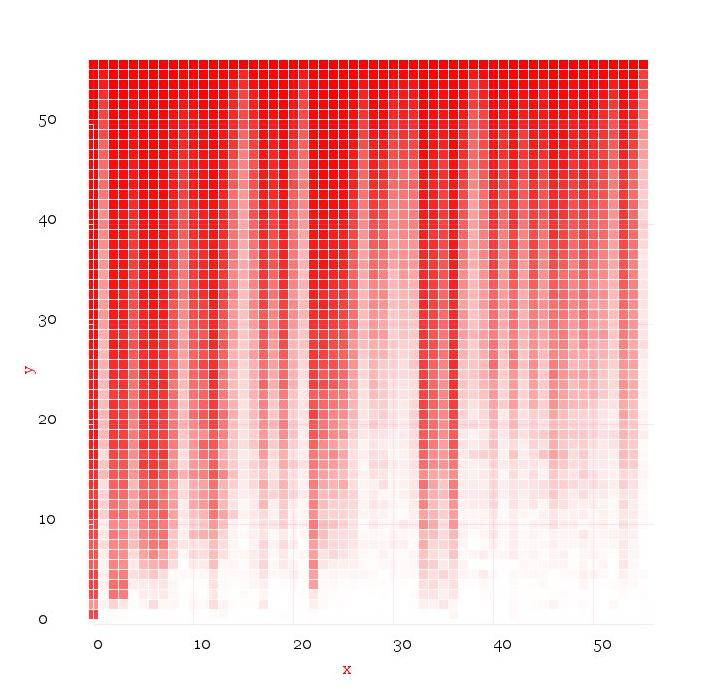
\includegraphics[width=120mm]{ReportMedia/AnswerDistribution.jpg}\\
\end{center}
\end{figure}
\subsubsection{Observations/Notes}
\begin{itemize}
\item The 'difficulty' metric of questions tends to clump together in bands in the left two-thirds of the map. Answering patterns from around question number 37 and above alternate much more uniformly.
\end{itemize}

\subsection{Effectiveness of intervention}
\subsubsection{Intervention effect on indivdual responses: McNemar's Test}
McNemar's test for matched pairs is used to measure statistical difference between two tests on matched pairs of data. Examples of matched pairs of data are:
\begin{itemize}
\item Test scores of siblings
\item Test scores before and after intervention of the same student.
\end{itemize}
The second point is aligned with the situation that we are dealing with. The two, disjoint, tests essentially are:
\begin{itemize}
\item Candidate answered 1 to the question.
\item Candidate answered 0 to the question.
\end{itemize}
Using this, we will be able to deduce whether the intervention had any significant effect on the response to a particular question across the entire population of students. This has the side-effect of allowing us to analyse this data in a fine-grained fashion.

\subsection{Modeling responses as Bernoulli trials}
There are $n$ students. All of them have answered either 0 or 1, to, say, question 3. We may restate this phenomenon and say that there were $n$ Bernoulli trials performed on question 3, each outcome being either true or false. The probability of the outcome is, say, $p$. The definition of 'true' and 'false' in this case is arbitrary, and does not need to specifically correspond to the perceived value of the answer.\\
Under these conditions, the phenomenon can be modelled as a Binomial Distribution. Formally, the binomial distribution is the discrete probability distribution of the number of successes in a sequence of $n$ independent yes/no experiments, each of which yields success with probability $p$.
The probability $p$ will be specific to each question, and can be estimated from the dataset.
Here is an example of the type of question that this modeling will be able to answer:\\\\
\textbf{If I choose 6000 students randomly from the population, what is the probability that at least 100 of them have answered 1 to question 45?
}
\subsubsection{The Binomial Distribution}
The binomial distribution for a random variable $S$ (in our case, the response to a particular question), for which $n$ experiments have been conducted is a discrete probability distribution given by:
\[P(S=k) =^{n}C_{r}.p^{k}.(1-p)^{n-k}\]
where:
\[^{n}C_{r} = {n!\over{k!(n-k)!}}\]
Table~\ref{BernoulliProbabilitiesPrePost} summarises the probabilities for the pre- and post-intervention answers.
\begin{longtable}{|c|c|c|c|}
	\hline
Index & $P_{pre}(Answer=1)$ &  $P_{post}(Answer=1)$\\
	\hline
1 & 0.9462283384301733 & 0.982233872142129 \\
2 & 0.5107397699140819 & 0.6418377748652978 \\
3 & 0.8927479248580166 & 0.963885248288918 \\
4 & 0.8855759429153924 & 0.9571137323430902 \\
5 & 0.7667831658657347 & 0.8963157128294743 \\
6 & 0.8795689529634484 & 0.9554754623561963 \\
7 & 0.8994466288044269 & 0.9667613222659094 \\
8 & 0.8741444590068443 & 0.9521625163826999 \\
9 & 0.7712246978302024 & 0.8880515508955876 \\
10 & 0.623452745012378 & 0.7670380078636959 \\
11 & 0.7710426678316586 & 0.9049803407601573 \\
12 & 0.8090505315275958 & 0.9207077326343381 \\
13 & 0.8611839231105286 & 0.9410950924712392 \\
14 & 0.7652905198776758 & 0.8864132809086938 \\
15 & 0.5783457113732343 & 0.744575506043396 \\
16 & 0.4260594145915247 & 0.5671326634629387 \\
17 & 0.5827144313382846 & 0.7254259501965924 \\
18 & 0.7672564438619485 & 0.8914009028687928 \\
19 & 0.662807630697539 & 0.7944881316440949 \\
20 & 0.7896097276831222 & 0.9197611766419106 \\
21 & 0.59188874326489 & 0.747051114023591 \\
22 & 0.4380369884957041 & 0.59247123926023 \\
23 & 0.8520824231833406 & 0.9350516965195864 \\
24 & 0.8316950633464395 & 0.9384010484927916 \\
25 & 0.8089413135284695 & 0.9293723605650211 \\
26 & 0.7880442696956459 & 0.9172491626620067 \\
27 & 0.6848332605213339 & 0.8484782292121742 \\
28 & 0.4887869520897044 & 0.6438401048492791 \\
29 & 0.6410004368719965 & 0.8189529634483763 \\
30 & 0.6163899810688801 & 0.7939420416484637 \\
31 & 0.49344692005242463 & 0.6865807485073541 \\
32 & 0.5105941459152469 & 0.7051114023591087 \\
33 & 0.5081913499344692 & 0.7071865443425076 \\
34 & 0.8340978593272171 & 0.9393840104849279 \\
35 & 0.780690257754478 & 0.9070190767438474 \\
36 & 0.7031454783748362 & 0.850116499199068 \\
37 & 0.8453109072375128 & 0.9269695645842435 \\
38 & 0.5957477792340178 & 0.7741735838066113 \\
39 & 0.44033056647735547 & 0.6132226590942187 \\
40 & 0.5306538517547692 & 0.7051842143585263 \\
41 & 0.7143221202854231 & 0.8831731469346148 \\
42 & 0.5657856414737149 & 0.7348551041211592 \\
43 & 0.6976481724188146 & 0.8690476190476191 \\
44 & 0.550203873598369 & 0.7196009902431921 \\
45 & 0.673074122615407 & 0.8979903888160768 \\
46 & 0.5836609873307121 & 0.7459953400320373 \\
47 & 0.7170889762632882 & 0.8698485510412116 \\
48 & 0.6857798165137615 & 0.8449104412407165 \\
49 & 0.6198485510412116 & 0.8022062035823504 \\
50 & 0.6704528906363769 & 0.8373379933012961 \\
51 & 0.6138779670889762 & 0.8026066695791466 \\
52 & 0.5696446774428425 & 0.7395878840832969 \\
53 & 0.4630479102956167 & 0.6245449250036406 \\
54 & 0.6854885685160914 & 0.8392675112858599 \\
55 & 0.5814038153487695 & 0.7639070918887433 \\
56 & 0.29219455366244357 & 0.3939493228484054 \\
\hline
\caption{Known probabilities of pre- and post-intervention scores}
\label{BernoulliProbabilitiesPrePost}
\end{longtable}

\subsection{Test for variable independence}
Hypothesis testing is one of the practices in classical statistics, where a proposition, or a null hypothesis is either rejected or not. Failure to reject a null hypothesis does not necessarily imply its acceptance. One of the questions we asked is whether any of the variables in the school dataset were independent of each other. To frame this in terms of a hypothesis test, we used the Chi-Square test.
\subsubsection{Chi-square test}
\textbf{Null hypothesis: Area and Improvement are NOT related.} \\
 For \textbf{area vs. improvement}\\
 Chi-Square statistic = 56499.4692602837\\
 X2 = 9652.9739\\
 Degrees of freedom = 9426\\
 \textbf{Null hypothesis rejected}\\c
\\
\textbf{Null hypothesis: Area and Pre-Score are NOT related.}\\
 For \textbf{area vs. pre-score}\\
 Chi-Square statistic = 58665.7089390644\\
 X2 = 8062.2959\\
 Degrees of freedom = 7855\\
 \textbf{Null hypothesis rejected}\\
\\
\textbf{Null hypothesis: Area and Post-Score are NOT related.}\\
 For \textbf{area vs. post-score}\\
 Chi-Square statistic = 38567.0016158761\\
 X2 = 8062.2959\\
 Degrees of freedom = 7855\\
 \textbf{Null hypothesis rejected}\\
\\
\textbf{Null hypothesis: Language and Post-Score are NOT related.}\\
 For \textbf{language vs. post-score}\\
 Chi-Square statistic = 280.234448946825\\
 X2 = 96.2166\\
 Degrees of freedom = 75\\
 \textbf{Null hypothesis rejected}\\
\\
\textbf{Null hypothesis: Language and Improvement are NOT related.}\\
 For \textbf{language vs. improvement}\\
 Chi-Square statistic = 232.464548410971\\
 X2 = 113.1452\\
 Degrees of freedom = 90\\
 \textbf{Null hypothesis rejected}\\
\\
\textbf{Null hypothesis: Language and Pre-Score are NOT related.}\\
 For \textbf{language vs. pre-score}\\
 Chi-Square statistic = 277.85501653079\\
 X2 = 96.2166\\
 Degrees of freedom = 75\\
 \textbf{Null hypothesis rejected}\\

\newpage
\section{Prediction and Classification}
\subsection{Decision Trees}
\subsection{Bayes classifier}
\subsection{Density estimators}
\subsubsection{Naive Bayes density}
\subsubsection{Kernel density estimation}
\subsubsection{Results}
\begin{figure}
\caption{Bayes posterior distribution of language from score improvement}
\label{BayesLanguageFromImprovement}
\begin{center}
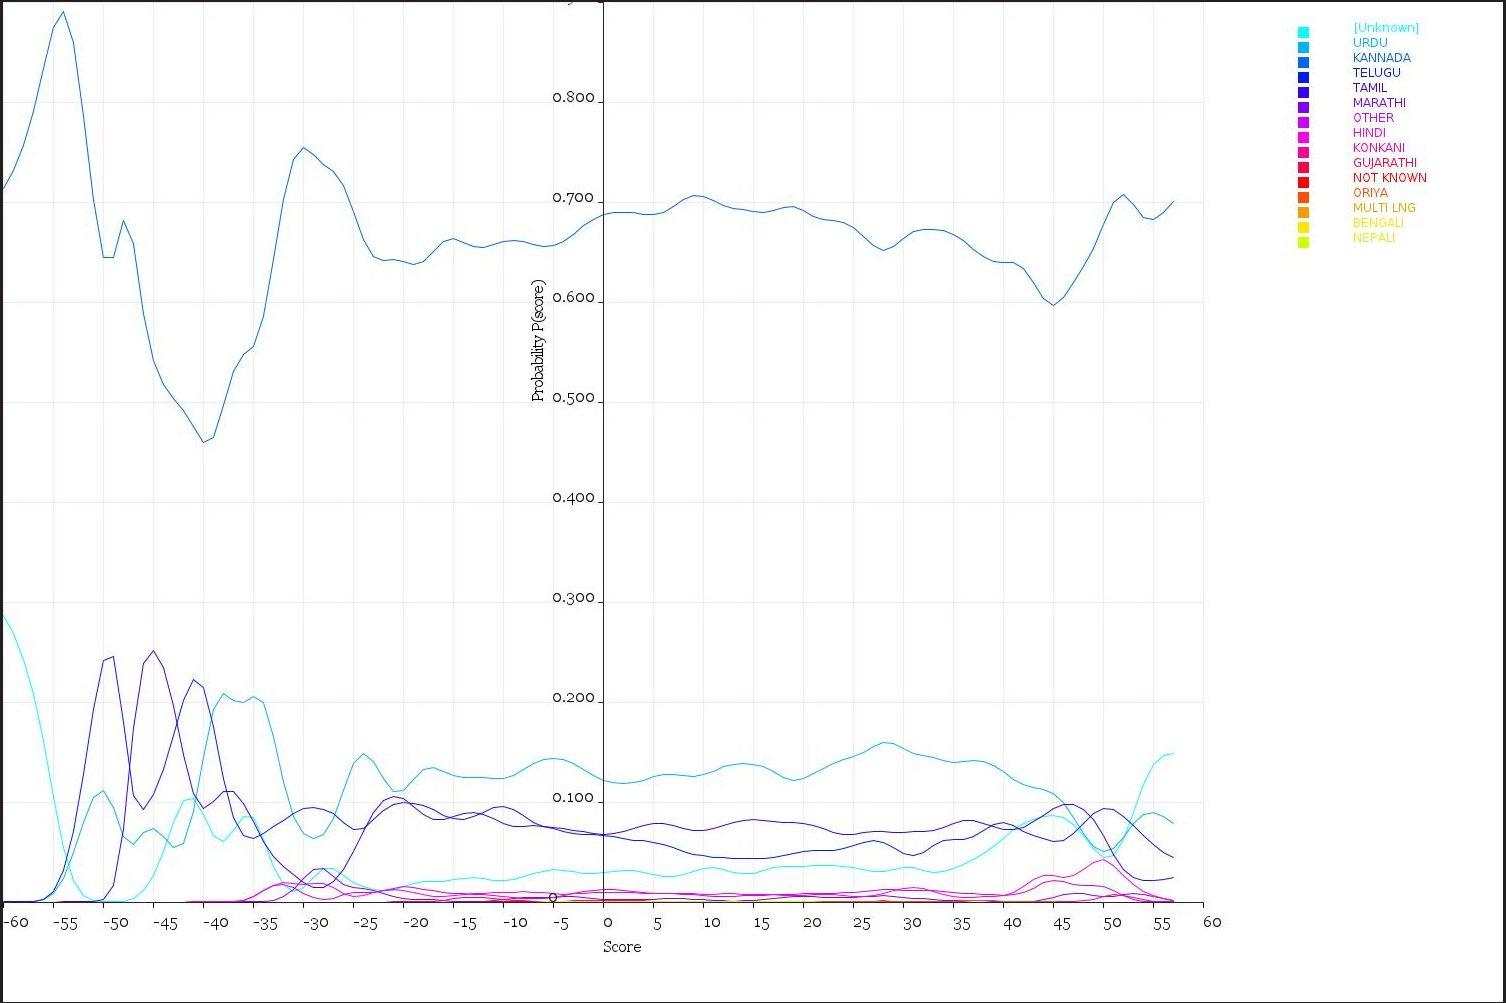
\includegraphics[width=160mm]{ReportMedia/BayesLanguageFromImprovement.jpg}\\
\end{center}
\end{figure}
\begin{figure}
\caption{Bayes posterior distribution of gender from score improvement}
\label{BayesGenderFromImprovement}
\begin{center}
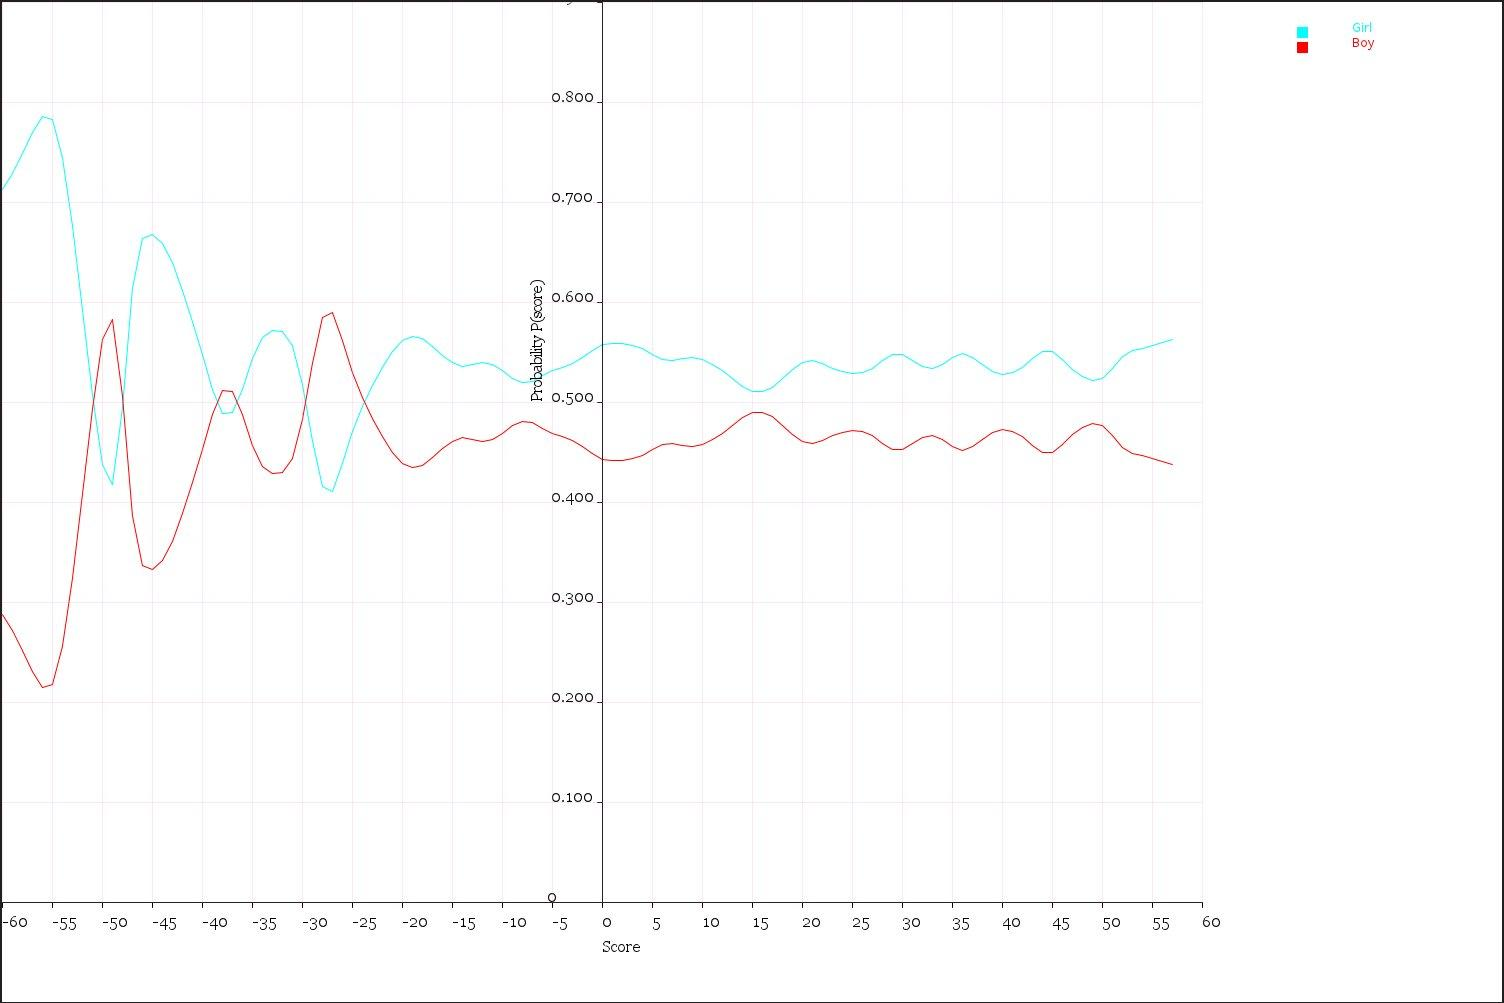
\includegraphics[width=160mm]{ReportMedia/BayesGenderFromImprovement.jpg}\\
\end{center}
\end{figure}
\begin{figure}
\caption{Bayes posterior distribution of geocluster from score improvement}
\label{BayesClusterFromImprovement}
\begin{center}
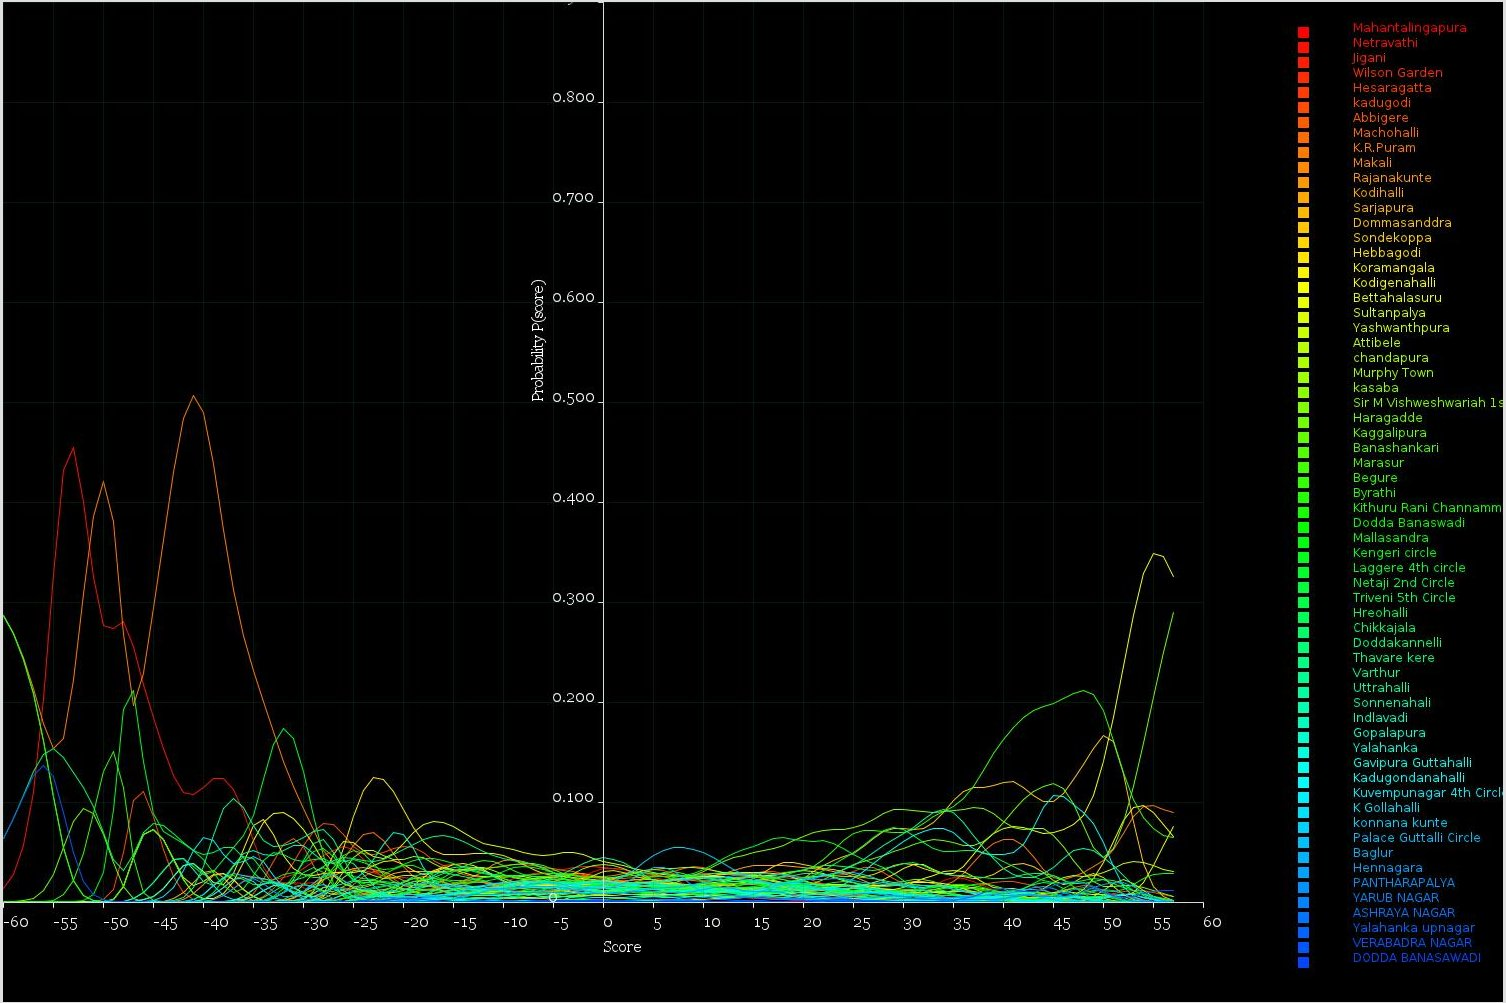
\includegraphics[width=160mm]{ReportMedia/BayesClusterFromImprovement.jpg}\\
\end{center}
\end{figure}
\newpage
\section{Dimension reduction/Factor analysis}
\subsection{Principal Component Analysis}

\newpage
\section{Technical notes}
For base visualisation and interactivity, Processing was used through its Ruby bindings (Ruby-Processing). All plots were done using a coordinate plotting gem called Basis-Processing.\\
Some calculations like Principal Component Analysis were done using the Statsample gem from the SciRuby project.\\
JRuby 1.6.4 was used for all code needing visualisation; Ruby 1.9.2 was used for everything else.\\
Data was stored in a MySQL database.
\end{document} 
